\documentclass[12pt,a4paper]{article}

% --------------------------------
% Пакеты для оформления и типографики
% --------------------------------
\usepackage[utf8]{inputenc}
\usepackage[russian]{babel}
\usepackage[T2A]{fontenc}
\usepackage{graphicx}
\usepackage{float}
\usepackage{xstring}
\usepackage{xparse}
\usepackage{caption}
\usepackage{geometry}
\usepackage{enumitem}
\usepackage{titlesec}
\usepackage{titletoc}    
\usepackage{etoolbox}     
\usepackage{tocloft}      
\usepackage{tikz}
\usetikzlibrary{patterns}
\usepackage{fancyhdr}
\usepackage{indentfirst}
\usepackage[colorlinks=true, linkcolor=black, urlcolor=blue, citecolor=blue]{hyperref}
\usepackage{xcolor}
\usepackage{pgfplots}
\usepackage{amsmath, amssymb, amsthm}
\pgfplotsset{compat=1.18}
\usetikzlibrary{positioning}
\usepackage{fancyhdr}
\usepackage{multirow}
\usepackage{array}
\pagestyle{fancy}
\fancyhf{}

% --------------------------------
% Колонтитулы
% --------------------------------
\fancyhead[L]{\leftmark}
\fancyhead[R]{\thepage}
\renewcommand{\sectionmark}[1]{\markboth{\textit{#1}}{}}
\geometry{margin=2.5cm} 
\setlength{\headwidth}{\textwidth}

% --------------------------------
% Геометрия страницы
% --------------------------------
\geometry{
    top=2.5cm,
    bottom=2.5cm,
    left=2.5cm,
    right=2.5cm
}

% --------------------------------
% Заголовки секций
% --------------------------------
\titleformat{\section}[block]{\normalfont\Large\bfseries}{\thesection.}{1em}{}
\titlespacing*{\section}{0pt}{3em}{1.5em}

\titleformat{\subsection}[block]{\normalfont\large\bfseries}{\thesubsection.}{1em}{}
\titlespacing*{\subsection}{0pt}{2em}{1.5em}

% --------------------------------
% Нумерация рисунков и таблиц
% --------------------------------
\captionsetup[figure]{labelfont=bf, name=Рисунок, labelsep=period}
\captionsetup[table]{labelfont=bf, name=Таблица, labelsep=period}

% --------------------------------
% Нумерованный список свойств
% --------------------------------

\newlist{deglist}{enumerate}{1}
\setlist[deglist]{label=\arabic*°., leftmargin=2em, itemsep=0.5em}

\newcommand{\deglistwithtitle}[2]{%
    \noindent\textbf{#1}\par\vspace{0.3em}
    \begin{deglist}
        #2
    \end{deglist}
}

% --------------------------------
% Оформление теорем, определений, замечаний
% --------------------------------
\theoremstyle{definition}
\newtheorem{definition}{Определение}[section]

\theoremstyle{definition}
\newtheorem{theorem}{Теорема}[section]

\newenvironment{proof}{
    \vspace{0.5em}
    \noindent\textit{Доказательство.}
}{\blacksquare\vspace{1em}}

\theoremstyle{remark}
\newenvironment{remark}{
  \par\noindent\textbf{\textit{Замечание.}}~
}{\par}

\theoremstyle{corollary}
\newenvironment{corollary}{
  \par\noindent\textbf{\textit{Следствие.}}~
}{\par}

\newcommand{\nextblock}{\vspace{1.5em}\noindent}

% --------------------------------
% Оформление типовых задач и решений
% --------------------------------
\newtheoremstyle{bolditalic}
  {\topsep}   % Space above
  {\topsep}   % Space below
  {\normalfont}  % Body font
  {}          % Indent amount
  {\bfseries\itshape} % Head font: bold italic
  {.}         % Punctuation after head
  { }         % Space after head
  {}          % Theorem head spec

\theoremstyle{bolditalic}
\newtheorem{example}{Пример}[section]

\newenvironment{solution}{
    \vspace{0.5em}
    \noindent\textit{Решение.}
}{\qed\vspace{1em}}

% --------------------------------
% Шаблон рисунков
% --------------------------------

\NewDocumentCommand{\myfigure}{O{0.75\textwidth} m m}{%
    \begin{figure}[H]
        \centering
        \includegraphics[width=#1]{#2}
        \caption{#3}
        \StrBefore{#2}{.}[\temp] % убираем расширение файла
        \label{fig:\temp}
    \end{figure}
}

% --------------------------------
% Начало документа
% --------------------------------
\begin{document}

\begin{center}
    {\LARGE \textbf{Методическое пособие по теории вероятностей}}\\[1em]
    {\large Мусатов И.А.}
\end{center}

\tableofcontents
\thispagestyle{empty}
\newpage

\section{Основы комбинаторики}

Комбинаторика --- основополагающий раздел математики, изучающий комбинации элементов некоторого конечного множества. Задачи, для решения которых используются комбинаторные методы, встречаются во многих разделах дискретной математики, в том числе и в дискретной вероятности.

В этой главе рассмотрим основные понятия комбинаторики.

\subsection{Принцип сложения и умножения}

\begin{definition}[Правило суммы]
Если некоторый объект класса A можно выбрать n способами, а другой объект класса B --- m способами, то выбор объекта <<A или B>> можно осуществить $n + m$ способами.
\end{definition}
\begin{example}
    В учебной группе состоят 12 девочек и 18 мальчиков. Требуется определить число возможных способов выбора старосты группы.
\end{example}
\begin{solution}
    Каждая из девочек может стать старостой. Тогда из класса объектов A имеем n = 12 способов выбора. Аналогично и с мальчиками: имеем m = 18 способов. Тогда, согласно правилу суммы, общее число способов выбора старосты равно $n + m = 30$.
\end{solution}
\begin{remark}
    При использовании правила суммы надо следить, чтобы способы выбора объектов A и B не пересекались. Иначе мы учтем какой-то выбор несколько раз. Поэтому в более общем случае формула выборки имеет вид: n + m - k, где k - число совпадающих способов выбора.
\end{remark}

\nextblock

\begin{definition}[Правило произведения]
Если объект класса A можно выбрать n способами и если после каждого такого выбора объект класса B можно выбрать m способами, то выбор упорядоченной пары (A, B) можно осуществить $n \cdot m$ способами.
\end{definition}

Для удобства восприятия данного правила можно воспользоваться мнемоникой <<корытец>>. Пусть в первое <<корытце>> можно положить объект n способами, во второе m, в третье k и так далее. Тогда общее число различных способов разложения равно произведению количеств способов для каждого <<корытца>>.

\myfigure[0.5\textwidth]{images/prod.png}{Мнемоника <<корытец>>}

\begin{example}
    Определить количество трехзначных чисел, в записи которых не встречаются цифры <<2>> и <<6>>.
\end{example}
\begin{solution}
    Рассмотрим трехзначное число как совокупность трех <<корытец>> для расположения цифр. Тогда на позицию первой цифры имеем 7 вариантов (всего цифр 10, но <<0>> не подходит по определению трехзначного числа, а <<2>> и <<6>> не подходят по условию). На позицию второй и третьей цифр подходят по 8 вариантов. Тогда по правилу произведения имеем: $7 \cdot 8 \cdot 8 = 448$ возможных трехзначных чисел, удовлетворяющих условию.
\end{solution}

\nextblock

В качестве более сложного примера рассмотрим задачу, где применяются правила как сложения, так и умножения.

\begin{example}
    Определить количество трехзначных чисел, в записи которых цифра <<2>> встречается ровно один раз.    
\end{example}
\begin{solution}
    Для начала из всех вариантов выделим взаимоисключающие случаи: когда цифра <<2>> располагается на первой позиции, когда располагается на второй и когда на третьей. Посчитаем для каждого случая число возможных способов в нем по правилу произведения. <<2>> на первой позиции: $1 \cdot 9 \cdot 9 = 81$ вариант, <<2>> на второй позиции: $8 \cdot 1 \cdot 9 = 72$ варианта, <<2>> на третьей позиции: $8 \cdot 9 \cdot 1 = 72$ варианта. Тогда, учитывая, что случаи взаимно исключают друг друга, общее число вариантов можем найти по правилу суммы: $81 + 72 + 72 = 225$ трехзначных чисел.
\end{solution}

\nextblock

Частным случаем правила произведения является размещение с повторением.

\begin{definition}[Размещения с повторениями] Числом размещений с повторениями из n по k (также известно как <<выборка с возвращением>>) называется число:
$$\overline{A}_n^k = n^k$$
\end{definition}

Обосновать данную формулу нетрудно. Полагая, что для каждого из k <<корытец>> у нас доступно n возможных предметов (причем предметы могут участвовать в размещении много раз), по правилу произведения действительно получаем $n \cdot n \cdot ... \cdot n = n^k$


\subsection{Базовые комбинаторные конфигурации}

Рассмотрим центральные понятия комбинаторики и их различия.

\begin{definition}[Перестановки]
Числом перестановок из $n$ называется число:
\[
P_n = n!
\]    
\end{definition}

Число перестановок --- это количество всех различных способов переставить данные n объектов между собой.
Понимать перестановки можно и через правило произведения. Пусть имеется конечное число объектов n, и требуется посчитать число их различных упорядочиваний друг за другом. Тогда на первую позицию можно поставить n объектов, на вторую n-1 (один объект уже поставлен), на третью n-2, ..., на n-ную 1 объект. Тогда общее число вариантов равно $n \cdot (n-1) \cdot (n-2) \cdot ... \cdot 1 = n!$.

\nextblock

Графическая иллюстрация принципа перестановок представлена на рисунке 2.

\myfigure[0.6\textwidth]{images/perm.png}{Иллюстрация перестановок}

\begin{example}
    На полке стоят 10 книг. Найти число таких расстановок, при которых конкретные 4 книги располагаются рядом.
\end{example}
\begin{solution}
    В данной задаче имеем ограничение на расстановку книг: конкретные 4 книги всегда должны стоять рядом. В таком случае временно <<свяжем>> эти 4 книги и будем рассматривать их как один объект. Тогда имеем $10 - 4 + 1 = 7$ объектов для свободной расстановки. Число их перестановок равно $7!$. Теперь вспомним, что внутри нашей <<связки>> книги также могут переставляться произвольно. Поэтому для каждого из $7!$ случаев можем рассматривать $4!$ перестановок внутри связки. Тогда по правилу произведения итоговое количество расстановок книг равно $P_7 \cdot P_4 = 7!\cdot4!=120960$.
\end{solution}

\begin{definition}[Размещения]
Числом размещений из $n$ по $k$ называется число: 
\[
A_n^k = \frac{n!}{(n-k)!}
\]
\end{definition}

Число размещений --- это количество всех различных способов расположить $n$ элементов по $k$ местам. При этом порядок расположения элементов \textbf{важен}. Т.е. расположения $(A\ B)$ и $(B\ A)$ в контексте размещений --- это \textbf{разные} случаи.

Можно заметить, что при $k = n$ формула $A_n^k$ обретает вид $A_n^n=n!$ и становится равной $P_n$. Действительно, если требуется разместить $n$ элементов на $n$ позиций, то мы имеем дело с их перестановками. Т.е. перестановки --- это частный случай размещений.

Формулу размещений также несложно вывести через правило произведения. Сначала преобразуем ее в удобную форму: $\frac{n!}{(n-k)!}=n\cdot(n-1)\cdot...\cdot(n-k+1)$. Получили произведение из $k$ сомножителей, каждый из которых на единицу меньше предыдущего. Т.е. мы постепенно из конечного набора из $n$ элементов $k$ раз достаем по одному произвольному элементу.

\nextblock

Графическая иллюстрация принципа размещений представлена на рисунке 3.

\myfigure[0.5\textwidth]{images/arrang.png}{Иллюстрация размещений}

\begin{example}
    Сколько существует чисел, в записи которых есть только нечетные цифры, причем никакая из цифр не встречается в числе дважды?
\end{example}
\begin{solution}
    Выпишем все нечетные цифры: $\{1, 3, 5, 7, 9\}$. Их 5. Значит, числа, удовлетворяющие условию, не могут иметь длину больше пяти. Тогда рассмотрим все длины от 1 до 5. В каждом из таких случаев (длина числа равна $i$) количество возможных способов составления числа равно $A_5^i$. Действительно: имеется конечный набор цифр, которые нужно расставить на позиции. Т.к. разные длины у одного числа --- это случаи несовместные, можем воспользоваться правилом суммы. Тогда итоговое количество чисел, удовлетворяющих условию, равно $A_5^1 + A_5^2 +...+A_5^5$ или же: $$\sum\limits_{i=1}^{5}{A_5^i}=325$$
\end{solution}

\begin{definition}[Сочетания]
Числом сочетаний из $n$ по $k$ называется число: 
\[
C_n^k = \frac{n!}{k!(n-k)!}
\]
\end{definition}

Число сочетаний --- это количество всех возможных способов выбора $k$ элементов из $n$ предложенных. При этом порядок расположения элементов в выборке \textbf{не важен}. Т.е. выборки $(A\ B)$ и $(B\ A)$ в контексте сочетаний --- это \textbf{одинаковые} случаи.

\nextblock

Сочетания можно себе представлять как размещения с намеренным исключением повторений. Пусть имеем размещения $A_n^k$. Тогда для каждого уникального набора конкретных $k$ объектов (скажем, набора $(A\ B\ C)$) в размещениях встречаются их все возможные перестановки ($(A\ B\ C)$, $(A\ C\ B)$, ..., $(C\ B\ A)$). Число таких перестановок нам известно. Это $P_k=k!$. Тогда, если мы хотим исключить такие повторения и для каждого уникального набора оставлять только одну <<неупорядоченную>> выборку, то достаточно общее число размещений поделить на число таких перестановок. В общем виде это выглядит как: $C_n^k=\frac{A_n^k}{k!}=\frac{n!}{k!(n-k)!}$.

\nextblock

Графическая иллюстрация принципа сочетаний представлена на рисунке 4.

\myfigure[0.5\textwidth]{images/comb.png}{Иллюстрация сочетаний}

\deglistwithtitle{Свойства сочетаний:}{
    \item $C_n^k = C_n^{n-k}$
    \item $C_n^0 = C_n^n = 1$
    \item $C_n^1=n$
    \item $C_n^2=\frac{n\cdot(n-1)}{2}$ --- также известно как <<число рукопожатий>>
    \item $C_n^k + C_n^{k-1} = C_{n+1}^k$
    \item $\sum\limits_{k=0}^{n}{C_n^k}=2^n$
}

\nextblock

\begin{example}
    В корзине лежат 5 яблок и 3 груши. Найти число способов достать четыре фрукта так, чтобы среди них было не менее двух груш.
\end{example}
\begin{solution}
    Т.к. в задаче присутствует неравенство (<<не менее двух груш>>), сразу разделим ее на несколько несовместных ситуаций. Груш не менее двух, значит, больше либо равно две. Но всего их три, а значит, представляются две ситуации: 1) берем две груши и два яблока; 2) берем три груши и одно яблоко. В первом случае по правилу произведения считаем число способов выбора: $C_3^2\cdot C_5^2=3\cdot10=30$. Во втором случае аналогично: $C_3^3\cdot C_5^1=1\cdot5=5$. Тогда по правилу суммы для несовместных выборок имеем итоговое число способов: $$C_3^2\cdot C_5^2+ C_3^3\cdot C_5^1=30+5=35$$
\end{solution}

\newpage

\section{Случайные события и вероятность}

\subsection{Понятие случайного события}

\begin{definition}
    \textbf{Случайным событием} называется явление, которое либо произойдет, либо не произойдет при наступлении некоторых указанных условий.
\end{definition}

<<Наступление указанных условий>> обычно кем-то производится намеренно. Поэтому будем называть <<наступление>> \textit{экспериментом} или \textit{испытанием}. 

\nextblock

\begin{remark}
    Случайные события обозначаются заглавными латинскими буквами
\end{remark}

\begin{definition}
    Событие называется \textbf{достоверным}, если оно обязательно произойдет в данном испытании.
\end{definition}

\begin{definition}
    Событие называется \textbf{невозможным}, если оно никогда не произойдет в данном испытании.
\end{definition}

\begin{definition}
    Два события $A$ и $B$ называются \textbf{несовместными}, если они не могут одновременно появиться в одном испытании. Т.е. появление одного из них исключает появление другого.
\end{definition}

\begin{definition}
    \textbf{Противоположным} к событию $A$ называется событие $\overline{A}$, которое заключается в отрицании появления $A$. Отличие от понятия <<несовместности>> в том, что в любом испытании всегда произойдет ровно одно из противоположных событий. В то время как несовместные события могут не возникнуть вовсе.
\end{definition}

\begin{definition}
    \textbf{Суммой} двух событий $A$ и $B$ называется событие $A+B$, которое возникает в случае наступления хотя бы одного из этих событий.
\end{definition}

\begin{definition}
    \textbf{Произведением} двух событий $A$ и $B$ называется событие $A\cdot B$, которое возникает только в случае, когда оба события наступили.
 \end{definition}

 Нетрудно заметить, что случайные события имеют теоретико-множественную природу. Т.е. операции над случайными событиями схожи с операциями над множествами. Соответственно, к арифметике случайных событий можно применять привычные законы коммутативности, ассоциативности, дистрибутивности, исключенного третьего, идемпотентности, де Моргана.

\begin{definition}
    События $A_1, A_2, ..., A_n$ образуют \textbf{полную группу}, если в результате испытания обязательно появится одно из них. Т.е. их сумма является достоверным событием.
\end{definition}

Например, события $A$ и $\overline{A}$ противоположны, следовательно, несовместны и образуют полную группу.

\subsection{Классическое определение вероятности}

\begin{definition}
    Элементарные исходы (результаты испытания), в которых интересующее нас случайное событие наступает, называются \textbf{благоприятствующими} данному событию.
\end{definition}

\begin{definition}[Классическое определение вероятности]
    Вероятность события $A$ равна отношению числа благоприятствующих этому событию исходов к общему числу всех исходов данного испытания. Обозначается как:
\[
P(A)=\frac{M}{N}
\]
\end{definition}

Из определения следует, что значение $P(A)$ лежит в промежутке $[0; 1]$. Где значение $0$ свидетельствует о невозможности события $A$, а значение $1$ --- о достоверности.

\begin{theorem}
    Вероятность суммы двух несовместных событий равна сумме их вероятностей:
    \[
    P(A+B)=P(A)+P(B)
    \]
\end{theorem}

\begin{theorem}
    Сумма противоположных событий равна $1$. Т.е. вероятность противоположного к $A$ события равна:
    \[
    P(\overline{A})=1-P(A)
    \]
\end{theorem}

\subsection{Типовая задача о выборке}

Нередко в статистике и математическом моделировании встречается задача, которую в общем виде можно описать следующим образом:

\begin{definition}[Задача о выборке]
    Имеется $N$ однородных предметов. $K$ из них <<особые>>. Произвольным образом из $N$ выбираются $n$ предметов. Определить вероятность того, что среди выбранных $n$ предметов ровно $k$ будут <<особыми>>. 
\end{definition}

\begin{solution}
    Решим задачу в общем виде. Для начала определим общее число возможных исходов. Имеется $N$ элементов, из них выбирается $n$, причем порядок не имеет значения. Значит, общее число исходов --- это число сочетаний $C_N^{n}$.\\\\
    Теперь найдем число благоприятствующих исходов. Т.е. таких случаев, когда среди выбранных $n$ предметов ровно $k$ <<особых>>. Раз число фиксировано, можно разбить задачу на две позадачи: выбрать $k$ <<особых>> предмета и $n-k$ не <<особых>>. Первая подзадача решается формулой выбора: $C_K^k$, вторая --- формулой выбора из оставшихся предметов: $C_{N-K}^{n-k}$. Понятно, что для каждого выбора в первой подзадаче может выпасть любой выбор из второй подзадачи. Значит, для вычисления общего числа благоприятствующих исходов можем воспользоваться правилом произведения, получив при этом: $C_K^k \cdot C_{N-K}^{n-k}$\\\\
    Тогда итоговая обобщенная формула для решения задачи о выборке имеет вид:
    \[
    P = \frac{C_K^k \cdot C_{N-K}^{n-k}}{C_N^{n}}
    \]
\end{solution}

\begin{example}
    В партии из 10 деталей 5 имеют отличное качество, 3 --- хорошее, а оставшиеся 2 --- бракованные. Случайным образом из партии выбираются 4 детали. Найти вероятность того, что среди выбранных деталей есть 2 отличного качества и одна бракованная.
\end{example}

\begin{solution}
    Общее число способов выбора 4 деталей из 10 равно $C_{10}^4$.\\
    Число благоприятных ситуаций --- это выборка 2х отличных деталей из 5 возможных, 1ой бракованной из 2 возможных, ну и оставшейся 1ой детали из 3 хороших. Тогда по правилу произведения можем представить это число как: $C_5^2\cdot C_2^1 \cdot C_3^1$.\\\\
    Следуя классическому определению вероятности, итоговая формула будет иметь вид:
    \[
    P = \frac{C_5^2\cdot C_2^1 \cdot C_3^1}{C_{10}^4} = \frac{2}{7}
    \]
\end{solution}

\subsection{Геометрическое определение вероятности}

Геометрические методы в математике всегда привлекают своей наглядностью. В теории вероятностей некоторые задачи также могут быть представлены в геометрической форме. Для этого достаточно ввести понятие \textit{меры}. Учитывая, что количество точек на любом отрезке и на любой площади бесконечно, мы прибегаем к таким конечным понятиям, как длина, площадь и объем. Для их обобщения и вводится понятие \textit{меры} как пространственного измерения отрезка, фигуры и тела в пространствах соответствующей размерности.

\begin{definition}[Геометрическое определение вероятности]
    Пусть $U$ --- область, соответствующая всем возможным элементарным исходам некоторого испытания. $A$ --- подобласть (не обязательно непрерывная) области $U$ , соответствующая всем благоприятствующим исходам. Тогда вероятность наступления случайного события соответствует вероятности попадания точки в область $A$, т.е. отношению мер областей:
    \[
    P(A) = \frac{\mu(A)}{\mu(U)}
    \]
\end{definition}

\begin{example}
    Дан отрезок $AB$ длины $L$. На нем произвольным образом отмечаются две точки: $M$ и $N$. Найти вероятность того, что длина получившегося отрезка $MN$ будет меньше, чем четверть длины исходного отрезка. 
\end{example}

\begin{solution}
    Имеем две точки, каждая из которых отмечается на отрезке независимо от другой. Тогда можем перейти к описанию каждой точки через определение переменных. Пусть $x$ отвечает за положение точки $M$, а $y$ --- за $N$. Тогда справедливо, что $0 \le x, y \le L$.\\
    Сформулируем теперь вопрос задачи, исползуя введенные переменные. Длина отрезка $MN$ через переменные определяется как $|y-x|$. Т.е. требуется найти $P\{|y-x|<L/4\}$\\\\
    Имея две переменные величины, можем перейти к геометрии на прямоугольной декартовой системе координат. Тогда пространством всех исходов станет квадрат с $0 \le x, y \le L$, а пространством благоприятствующих исходов --- $|y-x|<L/4 \iff y<x +L/4 \ \land y > x - L/4$. Изобразим это графически (см. рис. 5).\\
    Нетрудно посчитать площади указанных областей. Тогда итоговая  формула вероятности имеет вид:
    \[
    P\{[MN] < L/4\} = \frac{\mu(|y-x|<L/4)}{\mu(0 \le x, y \le L)} = \frac{7}{16}
    \]
\end{solution}

\begin{figure}[h]
\newcommand{\Lval}{8} % числовое значение L для построения
\centering
\begin{tikzpicture}[scale=0.8]

  % Штриховка области |y - x| < L/4
    \fill[green!30, opacity=0.6]
    (0, 0) --
    ({0 + \Lval/4}, 0) --
    (\Lval, {\Lval - \Lval/4}) --
    (\Lval, \Lval) --
    ({\Lval - \Lval/4}, \Lval) --
    (0, {\Lval/4}) -- cycle;

  % Квадрат
  \draw[thick] (0,0) rectangle (\Lval,\Lval);

  % Прямые y = x + L/4 и y = x - L/4
  \draw[dashed, thick] (0,{\Lval/4}) -- ({\Lval - \Lval/4},\Lval);
  \draw[dashed, thick] ({\Lval/4},0) -- (\Lval,{\Lval - \Lval/4});

  % Диагональ
  \draw[dashed] (0,0) -- (\Lval,\Lval);

  % Оси
  \draw[->] (-0.3,0) -- (\Lval + 0.7,0);
  \draw[->] (0,-0.3) -- (0,\Lval + 0.7);

  % Подписи осей и L
  \node at (-0.3,-0.3) {$0$};
  \node at (\Lval + 0.5,-0.3) {$x$};
  \node at (-0.3,\Lval + 0.5) {$y$};
  \node at (-0.5,\Lval - 0.2) {$L$};
  \node at (\Lval - 0.2,-0.5) {$L$};
  \node at (\Lval / 4, -0.5) {$L/4$};
  \node at (-0.5, \Lval / 4) {$L/4$};

  \node at (\Lval + 1, \Lval - \Lval / 4 + 0.5) {$y = x - L/4$};
  \node at (\Lval - \Lval / 4 + 0.5, \Lval + 0.5) {$y = x + L/4$};

\end{tikzpicture}
\caption{Область $\left| y - x \right| < \frac{L}{4}$}
\end{figure}

\begin{example}
    Даны два случайных действительных числа из отрезка $[0;2]$. Найти вероятность того, что произведение этих чисел будет больше 1.
\end{example}

\begin{solution}
    Обозначим числа за $x$ и $y$. Тогда условие задачи можно переписать в виде: $x, y \in \mathbb{R};\ 0 \le x, y \le 2;\ P\{x\cdot y>1\} - ?$.\\
    Перейдем к декартовой системе координат и изобразим области всех исходов и благоприятствующих исходов (см. рис. 6). Тогда вероятность может быть найдена как отношение площадей:\\
    \[
    \mu(x\cdot y > 1) = \frac{3}{2}\cdot2 - \int\limits_{0.5}^{2}{\frac{1}{x}dx}=3-\ln{x}{\Big|}_{0.5}^{2}=3-\ln{4}
    \]\\
    \[
    \mu(0 \le x, y \le 2) = 4
    \]\\
    \[
    P\{x\cdot y>1\}=\frac{\mu(x\cdot y > 1)}{\mu(0 \le x, y \le 2)} = \frac{3-\ln{4}}{4}
    \]
\end{solution}

\begin{figure}[h]
\centering
\begin{tikzpicture}[scale=3.2]

    \begin{scope}
    % Штриховка области между y=1/x и y=2
    \fill[pattern=north east lines, pattern color=blue, domain=0.5:2, variable=\x]
      (0.5,2) --
      plot ({\x}, {2}) -- 
      plot[domain=2:0.5] ({\x}, {1/\x}) -- cycle;
  \end{scope}    

  \draw[dashed, thick] (0.5,0) -- (0.5,2);
  \draw[dashed, thick] (0,0.5) -- (2,0.5);
  \draw[thick] (0,0) rectangle (2, 2);
  \draw[dashed, domain=0.5:2, smooth, variable=\x, blue, thick] plot ({\x}, {1/\x});

  % Оси
  \draw[->] (-0.3,0) -- (2+0.3,0) node[right] {$x$};
  \draw[->] (0,-0.3) -- (0,2+0.3) node[above] {$y$};

  \node at (-0.1,-0.1) {$0$};
  \node at (0.5,-0.2) {$\frac{1}{2}$};
  \node at (-0.2, 0.5) {$\frac{1}{2}$};
  \node at (-0.2, 2) {$2$};
  \node at (2,-0.2) {$2$};  

\end{tikzpicture}
\caption{Область $x\cdot y > 1$}
\end{figure}

\newpage

\subsection{Типовая задача о встрече}

Говоря о геометрическом определении вероятности, стоит рассмотреть отдельный класс задач, называемых задачами о встрече. Рассмотрим пример такой задачи.

\begin{example}[Задача о встрече]
    Два друга договорились о встрече в промежуток времени с 18:00 до 18:50. Причем условились, что каждый, придя на место встречи, будет ожидать другого не более, чем 20 минут. Найти вероятность того, что друзья \textbf{не} смогут встретиться.
\end{example}

\begin{solution}
    Анализируя условие, заметим, что нам не важна привязка начала промежутка времени к конкретному времени дня. Т.е. задача была эквивалентной, если бы они договорились встретиться в промежуток, скажем, с 12:40 до 13:30. Поэтому в задаче важен именно сам \textit{промежуток} времени, т.е. его продолжительность. В данном случае это 50 минут.\\\\
    На самом деле, подобную задачу мы уже рассматривали в примере 2.2. По сути, у нас есть отрезок (в данном случае времени), и две случайные точки (времена прибытия друзей). Можем так же ввести две переменные $0\le x, y \le 50$ --- случайное время прибытия от начала промежутка времени.\\\\
    Условие встречи друзей можно переформулировать как $|y-x| \le 20$. Т.е. разница между временами прихода друзей не превышает 20 минут. Тогда условие того, что они не встретятся --- $|y-x| > 20$.\\
    Получили условие, переведенное в удобную для построения на плоскости форму. Графическое решение представлено на рис. 7.\\
    А итоговая формула имеет вид:
    \[
    P\{|y-x|>20\} = \frac{\mu(|y-x|>20)}{\mu(0 \le x, y \le 50)} = \frac{9}{25}
    \]
\end{solution}

\begin{figure}[h]
\newcommand{\Lval}{8} % числовое значение L для построения
\centering
\begin{tikzpicture}[scale=0.8]

    \fill[red!30, opacity=0.6]
    (0.4*\Lval, 0) --
    (\Lval, 0) -- 
    (\Lval, 0.6 * \Lval) -- cycle;
    
    \fill[red!30, opacity=0.6]
    (0, 0.4*\Lval) --
    (0, \Lval) -- 
    (0.6 * \Lval, \Lval) -- cycle;

  % Квадрат
  \draw[thick] (0,0) rectangle (\Lval,\Lval);

  % Прямые y = x + L/4 и y = x - L/4
  \draw[dashed, thick] (0,{0.4*\Lval}) -- ({\Lval - 0.4*\Lval},\Lval);
  \draw[dashed, thick] ({0.4*\Lval},0) -- (\Lval,{\Lval - 0.4*\Lval});

  % Диагональ
  \draw[dashed] (0,0) -- (\Lval,\Lval);

  % Оси
  \draw[->] (-0.3,0) -- (\Lval + 0.7,0);
  \draw[->] (0,-0.3) -- (0,\Lval + 0.7);

  % Подписи осей и L
  \node at (-0.3,-0.3) {$0$};
  \node at (\Lval + 0.5,-0.3) {$x$};
  \node at (-0.3,\Lval + 0.5) {$y$};
  \node at (-0.5,\Lval - 0.2) {$50$};
  \node at (\Lval - 0.2,-0.5) {$50$};
  \node at (0.4*\Lval, -0.5) {$20$};
  \node at (-0.5, 0.4*\Lval) {$20$};

  \node at (\Lval + 1, \Lval - 0.4*\Lval + 0.5) {$y = x - 20$};
  \node at (\Lval - 0.4*\Lval + 0.5, \Lval + 0.5) {$y = x + 20$};

\end{tikzpicture}
\caption{Область $\left| y - x \right| > 20$}
\end{figure}

\newpage

\section{Условная вероятность и ее приложения}

\subsection{Операции над вероятностями}

\begin{theorem}[Теорема о сложении вероятностей]
    Вероятность суммы двух случайных событий равна сумме их вероятностей за вычетом вероятности их произведения:
    \[
    P(A+B)=P(A)+P(B)-P(A\cdot B)
    \]
\end{theorem}

\begin{remark}
    В частности, если $A$ и $B$ --- события несовместные, имеем: $P(A\cdot B) =0$. В таком случае вероятность их суммы: $P(A+B)=P(A)+P(B)$.
\end{remark}

\begin{definition}[Условная вероятность]
    Условной вероятностью $P(A|B)$ называют вероятность возникновения события $A$ при условии того, что событие $B$ уже произошло.\\\\
    Условная вероятность события $A$ также обозначается как: $P_B(A)$
\end{definition}

\begin{theorem}[Теорема о произведении вероятностей]
    Вероятность произведения двух случайных событий равна произведению вероятности первого события на условную вероятность второго:
    \[
    P(A\cdot B)=P(A)\cdot P(B|A)
    \]
\end{theorem}

\begin{definition}
    Случайное событие $B$ называют \textbf{независимым} от события $A$, если факт возникновения события $A$ не изменяет вероятности возникновения $B$:
    \[
    P(B|A)=P(B)
    \]
\end{definition}

\begin{corollary}
    Вероятность произведения независимых событий равна произведению их вероятностей:
    \[
    P(A\cdot B) = P(A) \cdot P(B)
    \]
\end{corollary}

\begin{definition}
    Вероятность появления хотя бы одного из независимых событий $A_1, A_2, ..., A_n$ противоположна произведению вероятностей непоявления каждого из событий:
    \[
    P(A_1 \lor A_2 \lor ... \lor A_n)=1-P(\bar{A_1})\cdot P(\bar{A_2})\cdot ... \cdot P(\bar{A_n})
    \]
\end{definition}

\begin{example}
    В первом мешке 5 белых и 9 черных шаров, а во втором --- 7 белых и 6 черных. Из каждого мешка вынули по одному шару.  Найти вероятность того, что вынутые шары будут разного цвета.
\end{example}

\begin{solution}
    Событие $A=$<<Вынутые шары разного цвета>> есть сумма двух несовместных событий: $A_1=$<<Первый вынутый белый, второй --- черный>> и $A_2=$<<Первый вынутый черный, второй --- белый>>.\\\\
    Событие $A_1$ --- это произведение двух независимых событий: $A_{11}=$<<Вынут белый из первого мешка>> $A_{12}=$<<Вынут черный из второго мешка>>. $P(A_{11})=5/14,\ P(A_{12})=6/13$. Т.о. $P(A_1)=P(A_{11})\cdot P(A_{12}) = \frac{5}{14} \cdot \frac{6}{13} = \frac{30}{182} $.\\\\
    Аналогично событие $A_2$ --- это произведение двух независимых событий: $A_{21}=$<<Вынут черный из первого мешка>> $A_{22}=$<<Вынут белый из второго мешка>>. $P(A_{21})=9/14,\ P(A_{22})=7/13$. Т.о. $P(A_2)=P(A_{21})\cdot P(A_{22}) = \frac{9}{14} \cdot \frac{7}{13} = \frac{63}{182} $.\\\\
    Событие $A$ --- сумма несовместных событий, значит, 
    \[
    P(A)=P(A_1)+P(A_2)=P(A_{11})\cdot P(A_{12})+P(A_{21})\cdot P(A_{22})=\frac{30}{182}+\frac{63}{182}=\frac{93}{182}
    \]
\end{solution}

\subsection{Типовая задача на надежность схем}

При создании электротехнических приборов в таких критических областях, как медицина, авионика, энергетика, жизненно важно учитывать все риски, которые могут нести в себе устройства. В качестве числовых характеристик для оценки надежности можно применять аппарат теории вероятностей. Ставится задача по вероятности надежности отдельных элементов вычислить надежность схемы в целом.\\

Рассмотрим основные соединения элементов в цепи:\\

\textbf{Последовательное соединение} работает исправно только если все элементы, в нем состоящие, работают исправно. На языке вероятности можем выразить это как: \[
P(AB)=P(A)\cdot P(B)
\]

\myfigure[0.35\textwidth]{images/scheme-seq.png}{Последовательное соединение}

\textbf{Параллельное соединение} работает исправно, если хотя бы один элемент такого соединения работает исправно. Иными словами, параллельное соединение не работает только в случае, когда не работают все элементы в нем. В таком случае на языке вероятности удобнее рассматривать надежность параллельного соединения от противного:
\[
P(A \lor B) = 1 - P(\bar{A})\cdot P(\bar{B})
\]

\myfigure[0.3\textwidth]{images/scheme-par.png}{Параллельное соединение}

\begin{remark}
    Определения надежности последовательного и параллельного соединений можно распространить и на произвольное число элементов.
\end{remark}

\begin{example}
    Определить надежность схемы, если известны вероятности безотказной работы ее элементов: $P(A)=0.6,\ P(B)=0.8$.
\end{example}

\myfigure[0.6\textwidth]{images/scheme.png}{Схема к примеру 3.2}

\begin{solution}
    Для начала вычислим надежности всех последовательных соединений на схеме. В нашем случае это: $AB,\ BB,\ AA$.
    \[
    P(AA)=P(A)\cdot P(A)=0.6\cdot0.6=0.36
\]\[
    P(AB)=P(A)\cdot P(B)=0.6\cdot 0.8 = 0.48
    \]
    \[
    P(BB)=P(B)\cdot P(B)=0.8\cdot 0.8 = 0.64
    \]
    Затем вычислим надежности параллельных соединений. В нашем случае имеется два параллельных соединения: $AB\ \lor BB$ и $B\lor A \lor AA$.
    \[
    P(AB \lor BB) = 1 - P(\overline{AB})\cdot P(\overline{BB})=1-(1-P(AB))\cdot (1-P(BB))=0.813
    \]
    \[
    P(B\lor A \lor AA)=1-P(\overline{B})\cdot P(\overline{A}) \cdot P(\overline{AA})= 1-(1-P(B))(1-P(A))(1-P(AA))=0.949
    \]
    В арифметике событий всю схему можно представить как:
    \[
    S = (AB\ \lor BB)\cdot(B\lor A \lor AA)
    \]
    Тогда вероятность ее надежности:
    \[
    P(S)=P((AB\ \lor BB)\cdot(B\lor A \lor AA))=P(AB\ \lor BB)\cdot P(B\lor A \lor AA)=0.813\cdot0.949=0.772
    \]
\end{solution}

\begin{remark}
    Зная надежность схемы, можем определить и вероятность ее отказа. Эти события противоположны, а значит, $P(\bar{S})=1-P(S)$.
\end{remark}

\subsection{Формула полной вероятности}

\begin{theorem}[Формула полной вероятности]
    Вероятность события $A$, которое может наступить только при условии появления одного из несовместных событий $H_1, H_2, ..., H_n$, образующих \textit{полную группу}, равна сумме произведений вероятности каждого из событий на условную вероятность события $A$:
    \[
    P(A) = P(A|H_1)\cdot P(H_1)+P(A|H_2)\cdot P(H_2)+...+P(A|H_n)\cdot P(H_n)
    \]
    Или:
    \[
    P(A)=\sum_{i=1}^{n}{P(A|H_i)\cdot p(H_i)}
    \]
\end{theorem}

\begin{remark}
    События $H_1, H_2, ..., H_n$ принято также называть \textbf{гипотезами}.\\\\
\textbf{Полной} такая вероятность называется потому, что рассматривает все возможные основания появления события $A$. Т.е. предполагает по отдельности каждую из гипотез, которые в совокупности составляют \textit{полную группу} (см. опр. 2.8).
\end{remark}

\begin{example}
    В соревнованиях участвовали 10 лыжников, 6 велосипедистов и 4 бегуна. Вероятность того, что лыжник выполнит свою норму, равняется 0.9, велосипедист --- 0.8, бегун --- 0.75. Определить вероятность события $A$ = <<Случайно выбранный спортсмен выполнит свою норму>>.
\end{example}

\begin{solution}
    Составим небольшую табличку по данному условию:
\begin{table}[h]
    \centering
    \begin{tabular}{|c|c|c|c|}
    \hline
     & \textbf{Лыж} & \textbf{Вел} & \textbf{Бег} \\
    \hline
    Кол-во & 10 & 6 & 4 \\
    \hline
    $P(A|H_i)$ & 0.9 & 0.8 & 0.75 \\
    \hline
    \end{tabular}
\end{table}

    Определим гипотезы, т.е. все возможные несовместные предпосылки события $A$:
    \vspace{1em}
    
    $H_1$ --- <<Выбранный спортсмен - лыжник>>
    
    $H_2$ --- <<Выбранный спортсмен - велосипедист>>
    
    $H_3$ --- <<Выбранный спортсмен - бегун>>\\
    \[
    P(H_1)=10/20=0.5
    \]
    \[
    P(H_2)=6/20=0.3
    \]
    \[
    P(H_3)=4/20=0.2
    \]

    Тогда по формуле полной вероятности:
    \[
    P(A) = P(A|H_1)\cdot P(H_1)+P(A|H_2)\cdot P(H_2)+P(A|H_3)\cdot P(H_3)=
    \]
    \[
    = 0.9\cdot 0.5 + 0.8\cdot 0.3 + 0.75\cdot 0.2=0.84
    \]
\end{solution}

\subsection{Формула Байеса}

\begin{theorem}[Формула Байеса]
    Пусть $A$ --- событие, которое может наступить только при осуществлении одной из гипотез полной группы ($H_1, ... H_n$). Тогда вероятность того, что событие $A$ осуществилось благодаря условию $H_i$, равна:
    \[
    P(H_i|A)=\frac{P(A|H_i)\cdot P(H_i)}{P(A)}
    \]
\end{theorem}

\begin{remark}
    Формулу Байеса также называют \textbf{формулой переоценки гипотез}.
\end{remark}
\vspace{1em}
Грубо говоря, формулу Байеса можно интерпретировать как взвешенную долю, которую вложила данная гипотеза в осуществление события $A$.

\begin{example}
    Для примера 3.3 найти вероятность того, что <<Спортсмен, выполнивший норму, является бегуном>>
\end{example}

\begin{solution}
    Значения $P(A), \ P(H_3), \ P(A|H_3)$ уже известны. Требуется только по формуле определить $P(H_3|A)$:
    \[
    P(H_3|A)=\frac{P(A|H_3)\cdot P(H_3)}{P(A)}=\frac{0.75\cdot 0.2}{0.84}=0.1786
    \]
\end{solution}

\newpage

\section{Повторные независимые испытания}

Общую постановку задач на повторные независимые испытания можно сформулировать следующим образом. Проводится $n$ однородных независимых испытаний, в результате каждого из которых событие $A$ может наступить или не наступить. Требуется определить вероятность того, что в $n$ испытаниях событие $A$ возникнет ровно $m$ раз: $P_n(m) - ?$.

\subsection{Формула Бернулли}

\begin{theorem}[Формула Бернулли]
    Пусть проводится конечное число $n$ испытаний, в каждом из которых событие $A$ может возникнуть с вероятностью $p$ и не возникнуть с вероятностью $q=1-p$. Тогда вероятность возникновения события $A$ ровно $m$ раз равна:
    \[
    P_n(m)=C_n^m\cdot p^m\cdot q^{n-m}
    \]
\end{theorem}

Формулу Бернулли нетрудно обосновать. Общая вероятность независимых событий равна произведению их вероятностей. Тогда раз мы имеем ровно $m$ событий с вероятностью $p$ и $n-m$ событий с вероятностью $q=1-p$, достаточно перемножить их соответствующее число раз. Но при этом не стоит также забывать, что мы не учли различные порядки следования успешности испытаний. Поэтому общую вероятность нужно домножить на число возможных конфигураций успешных событий. Оно равно числу выбора $m$ испытаний из $n$, т.е. числу сочетаний.

\begin{example}
    Вероятность попадания в мишень при одном выстреле равна 0.6. Было произведено 10 выстрелов.

    а) Найти вероятность того, что успешных выстрелов было ровно три;
    
    б) Найти вероятность того, что успешных выстрелов было не больше восьми;
\end{example}

\begin{solution}

    а) $P_{10}(3)=C_{10}^3\cdot 0.6^3\cdot 0.4^7=0.042$

    б) Можем пойти от вероятности противоположного события. <<Успешных выстрелов было больше 8>>. Тогда искомая вероятность: $P_{10}(\le8)=1-P_{10}(>8)=1-(P_{10}(9) + P_{10}(10))=1-(C_{10}^9\cdot 0.6^9\cdot 0.4+C_{10}^{10}\cdot 0.6^{10})=1-0.046=0.954$
\end{solution}

\subsection{Наивероятнейшее число появления события}

\begin{definition}[Наивероятнейшее число появления события]
    Наивероятнейшим числом появления события $A$ в $n$ испытаниях называется такое число $m^*$, вероятность $P_n(m^*)$ которого максимальна. Определяется через неравенство:
    \[
    (n+1)\cdot p - 1\le m^* \le (n+1)\cdot p
    \]
    То же, что и:
    \[
    np-q\le m^* \le np+p
    \]
\end{definition}

\begin{remark}
    Если обе границы неравенства являются целыми числами, то существует два наивероятнейших числа появления данного события.
\end{remark}

\begin{example}
    Имеется 8 станков. Вероятность исправной работы каждого из них равна 0.6. Определить, какое количество станков наиболее вероятно окажется исправным.
\end{example}

\begin{solution}
    Имеем: $n=8,\ p=0.6$. Тогда:
    \[
    9\cdot 0.6-1 \le m^* \le 9\cdot 0.6
    \]
    \[
    4.4 \le m^* \le 5.4
    \]
    \[
    m^*=5
    \]
\end{solution}

\begin{example}
    Вероятность выпуска прибора высшего качества составляет 0.75. Было выпущено 103 прибора. Определить наиболее вероятное число приборов высшего качества среди выпущенных.
\end{example}

\begin{solution}
    Имеем: $n=103,\ p=0.75$. Тогда:
    \[
    104\cdot 0.75-1 \le m^* \le 104\cdot 0.75
    \]
    \[
    77 \le m^* \le 78
    \]
    \[
    m^*=77,\ m^*=78
    \]
\end{solution}

\subsection{Теоремы Муавра-Лапласа}

При большом числе повторных независимых испытаний формула Бернулли вынуждает оперировать с числами значительно разных порядков (Так, скажем, уже при $n=10,\ m=7$: $10!=3\ 628\ 800$, а $0.2^7=0.0000128$. Что может стать причиной неустранимой погрешности вычислений. В целях минимизации данной погрешности используются локальная теорема Муавра-Лапласа и интегральная теорема Лапласа, дающие ассимптотическую формулу для нахождения приближенных значений вероятности.
\\

\begin{remark}
    Условие хорошего приближения данных теорем --- достаточно большое $n$. Чтобы дать этому численную характеристику, зададим условие: $n\cdot p\cdot q \ge 10$.
\end{remark}

\begin{theorem}[Локальная теорема Муавра-Лапласа]
    Если в каждом из $n$ независимых испытаний вероятность $p$ появления события $A$ постоянна, не равна 0 и 1, то вероятность возникновения события $A$ ровно $m$ раз приближенно равна:
     \[
     P_n(m) \approx \frac{1}{\sqrt{npq}}\cdot \varphi\left(\frac{m-np}{\sqrt{npq}}\right), 
     \]
     где $\varphi(x)=\frac{1}{\sqrt{2\pi}}\cdot e^{-x^2/2}\ $ --- функция Гаусса. $\varphi(-x)=\varphi(x);\ \varphi(\infty)=0$.
\end{theorem}

\begin{figure}[H]
\centering
\begin{tikzpicture}
\begin{axis}[
    width=12cm,
    height=7cm,
    axis lines = middle,
    xlabel = $x$,
    ylabel = {$f(x)$},
    grid = both,
    domain=-4:4,
    samples=200,
]
\addplot[
    very thick,
    black,
]
{1/sqrt(2*pi) * exp(-x^2/2)};
\end{axis}
\end{tikzpicture}
\caption{График функции Гаусса}
\end{figure}

\begin{remark}
    Значения функции Гаусса приведены в конце данного пособия в виде таблицы. 
\end{remark}

\begin{example}
    Монетка подбрасывается 324 раза. Определить вероятность того, что <<Орел>> выпадет ровно 172 раза.
\end{example}

\begin{solution}
    Вероятность выпадения <<Орла>> $p=0.5$. Проверим применимость локальной теоремы Муавра-Лапласа к данной задаче: $npq=324\cdot 0.5\cdot 0.5=81\ge10$. Тогда:
    \[
    P_{324}(172)=\frac{1}{\sqrt{npq}}\cdot\varphi\left(\frac{m-np}{\sqrt{npq}}\right)=\frac{1}{9}\cdot \varphi\left(\frac{172-162}{9}\right)=\frac{1}{9}\cdot \varphi(1.11)=0.024
    \]
\end{solution}


\begin{theorem}[Интегральная теорема Лапласа]
    Если в каждом из $n$ независимых испытаний вероятность $p$ появления события $A$ постоянна, не равна 0 и 1, то вероятность возникновения события $A$ не менее $m_1$, но не более $m_2$ раз приближенно равна:
    \[
    P_n\{m_1\le m\le m_2\} \approx \Phi\left(\frac{m_2-np}{\sqrt{npq}}\right) - \Phi\left(\frac{m_1-np}{\sqrt{npq}}\right),
    \]
    где $\Phi(x)=\frac{1}{\sqrt{2\pi}}\cdot\int\limits_{0}^{x}{e^{-t^2/2}dt}$ --- функция Лапласа. $\Phi(-x)=-\Phi(x);\ \Phi(\infty)=0.5;\ \Phi(0)=0$.
\end{theorem}

\myfigure[0.6\textwidth]{images/laplas-func.png}{График функции Лапласа}

\begin{remark}
    Значения функции Лапласа приведены в конце данного пособия в виде таблицы. 
\end{remark}

\begin{example}
    На потоке учатся 150 студентов. Вероятность того, что случайно взятый студент придет на лекцию по теории вероятностей --- 0.2. Найти вероятность того, что на лекции по теории вероятностей будет от 25 до 35 студентов.
\end{example}

\begin{solution}
    Проверим применимость интегральной теоремы Лапласа: $npq=150\cdot 0.2\cdot 0.8=24 \ge 10$. Тогда:
    \[
    P_{150}(25 \le m \le 35) = \Phi\left( \frac{35-150\cdot 0.2}{\sqrt{24}}\right)- \Phi\left( \frac{25-30}{\sqrt{24}}\right)=\Phi(1.02)-\Phi(-1.02)=
    \]
    \[
    =\Phi(1.02)+\Phi(1.02)=2\cdot \Phi(1.02)=0.69
    \]
\end{solution}

\begin{example}
    Вероятность того, что деталь из новой партии соответствует ГОСТ, составляет 0.8. Найти количество деталей в этой партии, если известно, что больше 78 деталей соответствуют ГОСТ с вероятностью 0.6915.
\end{example}

\begin{solution}
    По условию имеем: $p=0.8,\ q=0.2,\ P(78 \le m)=0.6915$.
    \[
    P(78 \le m)=\Phi(\infty)-\Phi\left(\frac{78-0.8\cdot n}{\sqrt{0.8\cdot 0.2n}}\right)=0.6915
    \]
    Знаем, что $\Phi(\infty)=0.5$. Тогда:
    \[
    \Phi\left(\frac{78-0.8\cdot n}{\sqrt{0.8\cdot 0.2n}}\right)=-0.1915 \iff \Phi\left(\frac{0.8\cdot n -78}{\sqrt{0.8\cdot 0.2n}}\right)=0.1915
    \]
    Смотрим значение аргумента по таблице:
    \[
    \frac{0.8\cdot n -78}{\sqrt{0.8\cdot 0.2n}}=0.5
    \]
    \[
    0.8n-78=0.2\sqrt{n}
    \]
    \[
    4n-\sqrt{n}-390=0
    \]
    \[
    n=100
    \]
\end{solution}

\subsection{Отклонение частоты от вероятности}

\begin{definition}
    Проводятся независимые испытания с постоянной вероятностью $p$ возникновения события $A$ в каждом из них. При этом в рамках данного эксперимента событие $A$ появилось $m$ раз в $n$ испытаниях. Тогда вероятность того, что отклонение относительной частоты $m/n$ от вероятности $p$ по модулю не превзойдет значения $\varepsilon$, приблизительно составляет:
    \[
    P\left\{\left|\frac{m}{n} - p\right| \le \varepsilon \right\} \approx 2\cdot \Phi\left( \varepsilon \cdot \sqrt{\frac{n}{pq}}\right)
    \]
\end{definition}

\begin{example}
    Проводятся измерения механического станка, изготавливающего качественные детали с вероятностью $p=0.8$. Вероятность того, что отклонение частоты от вероятности не превзойдет $\varepsilon=0.05$ составляет 0.95. Найти число проведенных испытаний $n$.
\end{example}

\begin{solution}
    Имеем: $p=0.8,\ P\left\{\left|\frac{m}{n} - 0.8\right| \le 0.05 \right\}=0.95$

    Определим $n$ исходя из формулы:
    \[
    P\{...\}=0.95\approx2\cdot \Phi\left( 0.05 \cdot \sqrt{\frac{n}{0.8\cdot0.2}}\right)
    \]
    \[
    \Phi\left( 0.05 \cdot \sqrt{\frac{n}{0.8\cdot0.2}}\right)=0.475
    \]
    \\
    Значение аргумента из таблицы функции Лапласа:
    \[
     0.05 \cdot \sqrt{\frac{n}{0.8\cdot0.2}}=1.96
    \]
    \[
    n=245.86\approx 246
    \]
\end{solution}

\subsection{Формула Пуассона}

Хоть локальная и интегральная формулы Муавра-Лапласа и хорошо приближают значение вероятности при большом числе испытаний, они, все же, дают большие погрешности при значениях вероятности, стремящихся к 1 или 0. В подобных ситуациях применяют ассимптотическую формулу Пуассона. 

\begin{theorem}[Формула Пуассона]
    Если число $n$ испытаний достаточно велико, а вероятность $p$ появления события $A$ в каждом испытании постоянна и близка к 0, то вероятность появления события $A$ ровно $m$ раз приближенно равна:
    \[
    P_n(m) \approx \frac{\lambda^m}{m!}\cdot e^{-\lambda}
    \]
    где $\lambda=n\cdot p$.
\end{theorem}

\begin{remark}
    Формула Пуассона дает хорошее приближение при небольших $\lambda$. Приблизительно $2 \le \lambda \le 9$.
\end{remark}

\begin{example}
    Высокоточный фрезерный ЧПУ-станок выпускает 1000 шестерней за смену. Вероятность того, что шестерня окажется бракованной, составляет 0.008. Определить вероятность того, что за смену ровно 5 деталей, выпущенных станком, окажутся бракованными.
\end{example}

\begin{solution}
    По условию: $n=1000,\ p=0.008$. $\lambda=np=8$.
    \[
    P_{1000}(5)=\frac{\lambda^m}{m!}\cdot e^{-\lambda}=\frac{8^5}{5!}\cdot e^{-8}=0.092
    \]
\end{solution}

\begin{example}
    В городе есть 200 книжных магазинов. Вероятность того, что студент в случайно выбранном магазине найдет книгу по функциональному анализу, составляет 0.01. Определить вероятность того, что студент сможет отыскать книгу хотя бы в двух магазинах.
\end{example}

\begin{solution}
    Имеем: $n=200,\ p=0.01$. $\lambda=np=2$. Требуется найти $P_n(m\ge2)$.
    Рассмотрим противоположное событие: студент сможет найти книгу меньше, чем в двух магазинах: $P_n(m < 2)=P_{200}(0)+P_{200}(1)$.
    \[
    P_{200}(0)=\frac{\lambda^m}{m!}\cdot e^{-\lambda}=\frac{2^0}{0!}\cdot e^{-2}=0.135
    \]
    \[
    P_{200}(1)=\frac{\lambda^m}{m!}\cdot e^{-\lambda}=\frac{2^1}{1!}\cdot e^{-2}=0.27
    \]
    Тогда вероятность исходного события:
    \[
    P_{200}(m\ge2)=1-P_{200}(m<2)=1-(P_{200}(0)+P_{200}(1))=1-0.405=0.595
    \]
\end{solution}

\newpage

\section{Случайные величины}

\subsection{Понятие случайной величины}

Для придания формальной характеристики результату испытания вводится такое понятие, как случайная величина. В общем виде это величина, которая в ходе испытания может принять одно значение из известного множества вероятных исходов.

\begin{remark}
    Случайные величины традиционно обозначаются греческими буквами ($\xi, \eta, \zeta, ... $), а их значения --- латинскими буквами ($x_i, y_i, z_i, ...$).
\end{remark}

\nextblock

По характеру множества допустимых значений случайные величины делят на дискретные и непрерывные.

\begin{definition}
    \textbf{Дискретной} называют случайную величину, которая принимает отдельные значения из конечного или бесконечного, но счетного множества.
\end{definition}

\begin{definition}
    \textbf{Непрерывной} называют случайную величину, которая принимает значения из числового промежутка: интервала, полуинтервала или отрезка (т.е. значения из несчетного множества).
\end{definition}

\begin{remark}
    В дальнейшем повествовании именование <<дискретные случайные величины>> будем сокращать до <<д.с.в.>>, а <<непрерывные случайные величины>> --- до <<н.с.в.>>.
\end{remark}

\subsection{Дискретные случайные величины}

\begin{definition}
    \textbf{Законом распределения} дискретной случайной величины $\xi$ называется соотношение между возможными значениями $x_i$ этой величины и соответствующими им вероятностями $p_i = P\{\xi=x_i\}$. Такое соотношение обычно выражается в виде таблицы:
    
    \centering
    \begin{tabular}{|c|c|c|c|c|}
    \hline
    $\xi$ & $x_1$ & $x_2$ & ... & $x_n$ \\
    \hline
    $p$ & $p_1$ & $p_2$ & ... & $p_n$ \\
    \hline
    \end{tabular}
\\
 
\end{definition}

\begin{remark}
    Закон распределения также называют рядом распределения или же просто распределением случайной величины.
\end{remark}

\nextblock

\begin{remark}
    Таблица является законом распределения случайной величины только если выполняется условие <<нормировки>>: сумма вероятностей должна быть равна 1. 
    \[
    \sum_{i=1}^{n}{p_i}=1
    \]
\end{remark}

\begin{definition}
    \textbf{Многоугольником распределения} называется график закона распределения. Т.е. откладывание значений случайной величины по оси Ox, а вероятностей --- по оси Oy.
\end{definition}

\begin{example}
    Имеется закон распределения д.с.в. $\xi$. Требуется построить многоугольник ее распределения.\\
    
    \centering
    \begin{tabular}{|c|c|c|c|c|}
    \hline
    $\xi$ & -1 & 0 & 2 & 5 \\
    \hline
    $p$ & 0.2 & 0.5 & 0.1 & 0.2 \\
    \hline
    \end{tabular}\\
\end{example}

\nextblock

\begin{solution}
    Перенесем данные из таблицы на график.\\  
    
    \begin{figure}[h!]
    \centering
    \includegraphics[width=0.5\linewidth]{}
    \begin{tikzpicture}
    \begin{axis}[
        axis lines   = middle,
        xlabel       = {$x_i$},
        ylabel       = {$P\{\xi = x_i\}$},
        ymin         = 0,      ymax = 0.6,
        xtick        = {-1,0,2,5},
        ytick        = {0,0.1,0.2,0.5},
        grid         = both,   minor grid style={dotted},
        width=10cm,  height=6cm
    ]
    
    % вертикальные «столбики»
    \addplot [ycomb, thick] coordinates {
        (-1,0.2) (0,0.5) (2,0.1) (5,0.2)
    };
    
    % сам многоугольник
    \addplot [thick, mark=*] coordinates {
        (-1,0.2) (0,0.5) (2,0.1) (5,0.2)
    };
    
    \end{axis}
    \end{tikzpicture}

    \caption{Многоугольник распределения д.с.в. $\xi$}
    \end{figure}
\end{solution}

\nextblock

\begin{definition}
    \textbf{Функцией распределения} $F(x)$ случайной величины $\xi$ называется вероятность того, что случайная величина будет меньше указанного аргумента:
    \[
    F(x)=P\{\xi<x\}
    \]
\end{definition}

\begin{remark}
    Т.к. функция распределения в каждой точке равна соответствующей вероятности, то естественно ожидать, что ее значения будут лежать в диапазоне от 0 до 1.
\end{remark}

\begin{remark}
    Функция распределения обладает свойством \textit{кумулятивности}. Т.е. значение функции от большего аргумента будет включать в себя значение от меньшего аргумента. Или же можно сказать, что значение функции постепенно <<накапливается>>, представляя собой префиксную сумму. Такое свойство особенно полезно для работы с диапазонами значений случайной величины, т.к. вероятность попадания на промежуток равна разности значений функции распределения на его концах.
\end{remark}

\nextblock

\deglistwithtitle{Свойства функции распределения:}{
    \item $0 \le F(x) \le 1$
    \item $F(-\infty)=0; F(+\infty)=1$
    \item $P\{x_1 \le \xi < x_2\} = F(x_2) - F(x_1)$
    \item $F(x)$ --- неубывающая функция
    \item $F(x)$ --- непрерывна слева
}

\begin{example}
     Для д.с.в. $\xi$, заданной следующим законом распределения, определить функцию распределения, построить ее график, а также найти вероятность попадания $\xi$ на интервал $(1;7)$.\\
    
    \centering
    \begin{tabular}{|c|c|c|c|c|}
    \hline
    $\xi$ & -1 & 0 & 2 & 5 \\
    \hline
    $p$ & 0.2 & 0.5 & 0.1 & 0.2 \\
    \hline
    \end{tabular}\\
\end{example}

\begin{solution}
    Пользуясь определением 5.5, составим кусочную функцию распределения д.с.в. $\xi$:
    \[
    F(x) = \begin{cases}
      0, & x \le -1 \\
      0.2, & -1 < x \le 0 \\
      0.7, & 0 < x \le 2 \\
      0.8, & 2 < x \le 5 \\
      1, & x > 5 \\
    \end{cases}
    \]

    По аналитическому заданию функции нетрудно построить ее график:

    \begin{figure}[h!]
        \centering
        \includegraphics[width=0.5\linewidth]{}
\begin{tikzpicture}
\begin{axis}[
    axis lines = middle,
    xlabel = {$x$},
    ylabel = {$F(x)$},
    xmin = -2, xmax = 7,
    ymin = -0.1, ymax = 1.1,
    xtick = {-2,-1,0,1,2,3,4,5,6,7},
    ytick = {0,0.1,0.2,0.7,0.8,1},
    grid = both,
    major grid style = {gray!30, dashed},
    minor tick num = 1,
    minor grid style = {dashed, gray!30},
    width = 12cm,
    height = 7cm,
    samples = 200,
    domain = -2:7
]

% Ступенчатый график F(x)
\addplot [
    thick,
    domain=-2:-1,
] {0};

\addplot [
    thick,
    domain=-1:0,
] {0.2};

\addplot [
    thick,
    domain=0:2,
] {0.7};

\addplot [
    thick,
    domain=2:5,
] {0.8};

\addplot [
    thick,
    domain=5:7,
] {1};

% Пустые и закрашенные точки на ступенях
\addplot[only marks, mark=*, mark size=2pt] coordinates {(-1, 0)};
\addplot[only marks, mark=*, fill=white, mark size=2pt] coordinates {(-1, 0.2)};
\addplot[only marks, mark=*, mark size=2pt] coordinates {(0, 0.2)};
\addplot[only marks, mark=*, fill=white, mark size=2pt] coordinates {(0, 0.7)};
\addplot[only marks, mark=*, mark size=2pt] coordinates {(2, 0.7)};
\addplot[only marks, mark=*, fill=white, mark size=2pt] coordinates {(2, 0.8)};
\addplot[only marks, mark=*, mark size=2pt] coordinates {(5, 0.8)};
\addplot[only marks, mark=*, fill=white, mark size=2pt] coordinates {(5, 1)};

\end{axis}
\end{tikzpicture}
        \caption{График функции распределения д.с.в. $\xi$}
    \end{figure}


    Теперь найдем вероятность попадания $\xi$ на интервал $(1;7)$. Для этого достаточно найти разность значений функции распределения:
    \[
    P\{\xi \in (1;7)\} = P\{1< \xi <7\}=P\{\xi < 7\} - P\{\xi < 1\} = F(7)-F(1)=1-0.7=0.3
    \]
\end{solution}

\subsection{Числовые характеристики д.с.в}

Для извлечения определенной информации о случайных величинах традиционно используют несколько числовых характеристик: математическое ожидание, дисперсия, среднее квадратическое отклонение, корреляционный момент (ковариация).

\begin{definition}
    \textbf{Математическим ожиданием} $M(\xi)$ дискретной случайной величины $\xi$ называют взвешенную сумму ее значений (сумму произведений значений на соответствующие вероятности):
    \[
    M(\xi)= \sum_{i=1}^{n}{x_i \cdot p_i}
    \]
\end{definition}

\begin{remark}
    В некоторых источниках можно встретить и другие обозначения для математического ожидания: $M_\xi, E[\xi]$.
\end{remark}
\begin{remark}
    Математическое ожидание стоит понимать как средневзвешенное значение случайной величины. Т.е. ее наиболее <<ожидаемое>> значение. 
\end{remark}

\nextblock

\deglistwithtitle{Свойства математического ожидания:}{
    \item $M(C)=C$, где C - константа
    \item $M(C\cdot \xi)=C\cdot M(\xi)$ --- вынос константы
    \item $M(\xi + \eta)=M(\xi)+M(\eta)$ --- свойство линейности
    \item $M(\xi \cdot \eta)=M(\xi)\cdot M(\eta)$ --- только для независимых с.в. $\xi$ и $\eta$
}

\nextblock

\begin{definition}
    \textbf{Дисперсией} случайной величины называется математическое ожидание квадрата ее отклонения от математического ожидания:
     \[
     D(\xi)=M[(\xi-M(\xi))^2]
     \], или же:
     \[
     D(\xi)=M(\xi^2)-(M(\xi))^2
     \]
     Для дискретной с.в. справедлива также формула:
     \[
     D(\xi)=\sum_{i=1}^{n}{(x_i-M(\xi))^2\cdot p_i}
     \]
\end{definition}

\begin{remark}
    Для оценки степени <<разброса>> с.в. относительно ее мат.ожидания нецелесообразно рассматривать разницу с.в. и мат.ожидания, т.к. в среднем такая разница в силу случайности равна нулю. Чтобы предотвратить такое обнуление, изучают мат.ожидание квадрата отклонения. Таким образом, дисперсия представляет собой ожидаемое значение квадрата отклонения. Т.е. это величина квадратичная.
\end{remark}

\nextblock

\deglistwithtitle{Свойства дисперсии:}{
    \item $D(\xi) \ge 0$
    \item $D(C) = 0$, где C --- константа
    \item $D(C\cdot \xi)=C^2\cdot D(\xi)$
    \item $D(\xi + \eta) = D(\xi) + D(\eta) + 2\cdot K(\xi, \eta)$, где $K$ --- ковариация с.в. $\xi$ и $\eta$
    \item $D(\xi + \eta) = D(\xi) + D(\eta)$ --- для независимых с.в. $\xi$ и $\eta$
}

\nextblock

\begin{definition}
    \textbf{Средним квадратическим отклонением} случайной величины $\xi$ называют квадратный корень из ее дисперсии:
    \[
    \sigma(\xi)=\sqrt{D(\xi)}
    \]
\end{definition}

\begin{remark}
    Среднее квадратическое отклонение --- это прямая характеристика среднего отклонения величины от ее математического ожидания. Основной ожидаемый разброс значений с.в. будет располагаться на интервале $(M_\xi - \sigma_\xi; M_\xi + \sigma_\xi)$.
\end{remark}

\nextblock

\begin{definition}
    \textbf{Ковариацией} (корреляционным моментом) двух случайных величин $\xi$ и $\eta$ называется математическое ожидание произведения <<центрированных>> случайных величин $\xi$ и $\eta$:
    \[
    K(\xi, \eta) = M[(\xi-M(\xi))\cdot(\eta-M(\eta))]
    \], или же
    \[
    K(\xi, \eta) = M(\xi \cdot \eta) - M(\xi)\cdot M(\eta)
    \]
\end{definition}

\begin{remark}
    В некоторых источниках ковариация также может обозначаться как $cov(\xi, \eta)$.
\end{remark}
\begin{remark}
    Ковариация показывает степень созависимости случайных величин. Т.е. то, насколько значения одной случайной величины влияют на значение другой. Если случайные величины заведомо независимы, то их ковариация равна нулю. Более подробно эту числовую характеристику рассмотрим в главе <<двумерные случайные величины>>.
\end{remark}

\nextblock

\begin{example}
    Для д.с.в. $\xi$, заданной следующим законом распределения, определить математическое ожидание, дисперсию, среднее квадратическое отклонение, а также найти ковариацию $\xi$ с постоянной случайной величиной: $\eta = 5$.\\
    
    \centering
    \begin{tabular}{|c|c|c|c|c|}
    \hline
    $\xi$ & -1 & 0 & 2 & 5 \\
    \hline
    $p$ & 0.2 & 0.5 & 0.1 & 0.2 \\
    \hline
    \end{tabular}\\
\end{example}
\begin{solution}
    Согласно формуле мат.ожидания для д.с.в. имеем:
     \[
     M(\xi) = \sum_{i=1}^{n}{x_i \cdot p_i} = -1\cdot0.2+0\cdot0.5+2\cdot0.1+5\cdot0.2=1
     \]
    Для нахождения дисперсии посчитаем мат.ожидание квадрата случайной величины:
     \[
     M(\xi^2) = \sum_{i=1}^{n}{x_i^2 \cdot p_i} = (-1)^2\cdot0.2+0^2\cdot0.5+2^2\cdot0.1+5^2\cdot0.2=5.6
     \]
     Теперь можем вычислить дисперсию по упрощенной формуле:
    \[
    D(\xi)=M(\xi^2)-(M(\xi))^2 = 5.6-1^2=4.6
    \]
    Среднее квадратическое отклонение:
    \[
    \sigma(\xi)=\sqrt{D(\xi)} = \sqrt{4.6} \approx 2.1448
    \]
    Для вычисления ковариации сначала вычислим мат.ожидание произведения случайных величин. Для этого рассмотрим все возможные комбинации значений с.в. и их вероятности. Т.к. величина $\eta$ постоянна и имеет значение 5 с вероятностью 1, достаточно будет рассмотреть только четыре ситуации:\\
    
    \begin{center}
    \begin{tabular}{|c|c|c|c|c|}
    \hline
    $\eta$ & 5 & 5 & 5 & 5 \\
    \hline
    $\xi$ & -1 & 0 & 2 & 5 \\
    \hline
    $p$ & 0.2 & 0.5 & 0.1 & 0.2 \\
    \hline
    \end{tabular}
    \end{center}\\

    Математическое ожидание произведения с.в. вычисляется как:
    \[
    M(\xi\cdot \eta)=\sum_{i=1}^{n}{\sum_{j=1}^{m}{x_i\cdot y_j \cdot p_{ij}}}=5\cdot (-1\cdot0.2+0\cdot0.5+2\cdot0.1+5\cdot0.2)=5
    \]
    Математическое ожидание константной случайной величины $\eta$: 
    \[
    M(\eta)=M(5)=5
    \]
    Тогда ковариация:
    \[
    K(\xi, \eta)=M(\xi \cdot \eta) - M(\xi)\cdot M(\eta)=5-1\cdot5=0
    \]
    Такой же результат можно было бы получить из факта независимости данных с.в. 
\end{solution}


\subsection{Непрерывные случайные величины}

\begin{definition}
    Случайная величина $\xi$ называется \textit{непрерывной}, если ее функция распределения $F(x)$ непрерывна и обладает кусочно-непрерывной производной $F'(x)$.
\end{definition}

Вероятность попадания непрерывной случайной величины в заданный промежуток зависит от скорости роста функции распределения. Поэтому непрерывную случайную величину задают при помощи производной от функции распределения. 

\begin{definition}
    \textbf{Плотностью распределения} $f(x)$ н.с.в. $\xi$ называют первую производную от ее функции распределения:
    \[
    f(x) = F'(x)
    \]
\end{definition}

\begin{remark}
    Плотность распределения --- основная характеристика непрерывных случайных величин. По своему значению она эквивалентна закону распределения у дискретных случайных величин, обеспечивая меру вероятности для значений случайной величины. 
\end{remark}

\nextblock

\deglistwithtitle{Свойства плотности распределения:}{
    \item $f(x) \ge 0$ --- плотность не может вносить отрицательную вероятность
    \item $f(-\infty)=f(+\infty)=0$
    \item $f(x)$ --- кусочно-непрерывная функция
    \item $F(x) = \int\limits_{-\infty}^{x}{f(t)dt}$ --- определение функции распределения через плотность
    \item $P\{x_1 \le \xi < x_2\}=\int\limits_{x_1}^{x_2}{f(x)dx}$ --- вычисление вероятности через плотность
    \item $\int\limits_{-\infty}^{+\infty}{f(x)dx} = 1$ --- условие нормировки плотности
}

\nextblock

\begin{example}
    Непрерывная случайная величина $\xi$ задана функцией распределения:\\

    \[
    F(x) = \begin{cases}
      0, & x \le 0 \\
      0.25\cdot x^2, & 0 < x \le 2 \\
      1, & x > 2 \\
    \end{cases}
    \]
    \\
    
    Требуется найти функцию плотности н.с.в. и проверить результат условием нормировки. Определить вероятность того, что случайная величина $\xi$ примет значение из интервала $(1;3)$
\end{example}
\begin{solution}
    Функция плотности представляет собой первую производную функции распределения. Поэтому на каждом промежутке кусочного определения найдем производную: для $x \le 0$ это $0' = 0$, для $0 < x \le 2$ производная: $(0.25\cdot x^2)'= 0.5\cdot x$, для $x > 2$ это $1' = 0$. Т.о.:\\
    \[
    f(x) = \begin{cases}
      0, & x \le 0 \\
      0.5\cdot x & 0 < x \le 2 \\
      0, & x > 2 \\
    \end{cases}
    \]

    Проверим корректность нахождения функции плотности при помощи условия нормировки:
    \[
    \int\limits_{-\infty}^{+\infty}{f(x)dx} = 1
    \]
    \[
    \int\limits_{-\infty}^{+\infty}{f(x)dx} = \int\limits_{-\infty}^{0}{f(x)dx} + \int\limits_{0}^{2}{f(x)dx} + \int\limits_{2}^{+\infty}{f(x)dx}=
    \]
    \[
    =\int\limits_{-\infty}^{0}{0\cdot dx} + \int\limits_{0}^{2}{0.5\cdot xdx} + \int\limits_{2}^{+\infty}{0\cdot dx}=0+\left(0.25\cdot x^2\right){\Big|}_{0}^{2}+0=1
    \]
    Т.о., условие нормировки соблюдено.\\
    \\
    Вероятность того, что $\xi$ примет значение из интервала $(1;3)$:
    \[
    P\{\xi\in(1;3)\}=P\{1<\xi<3\}=\int\limits_{1}^{3}{f(x)dx}=\int\limits_{1}^{2}{f(x)dx}+\int\limits_{2}^{3}{f(x)dx}=
    \]
    \[
    = \int\limits_{1}^{2}{0.5\cdot x dx} + \int\limits_{2}^{3}{0\cdot dx}=\left(0.25\cdot x^2\right){\Big|}_{1}^{2} + 0=1-0.25 = 0.75
    \]
\end{solution}

\begin{example}
    Задана функция распределения н.с.в. $\xi$:\\
    
    \[
    F(x) = \begin{cases}
      0, & x \le -1 \\
      A\cdot(x^3+1), & -1 < x \le 3 \\
      1, & x > 3 \\
    \end{cases}
    \]
    \\
    Найти значение параметра A и вероятность того, что случайная величина $\xi$ примет значение из интервала $(-2;2)$. Построить график функции распределения.
\end{example}
\begin{solution}
    Функция распределения н.с.в. обязательно должна быть непрерывной. Исходя из этого факта, определим параметр А так, чтобы односторонние пределы функции в окрестности $x=3$ были равны, тем самым обеспечивая непрерывность функции:
    \[
    \lim_{x\rightarrow3-0}{A\cdot(x^3+1)} = \lim_{x\rightarrow3+0}{1}
    \]
    \[
    A\cdot (27 + 1)=1
    \]
    \[
    A = \frac{1}{28}
    \]
    Т.о., функция распределения имеет вид:

    \[
    F(x) = \begin{cases}
      0, & x \le -1 \\
      \frac{1}{28}\cdot(x^3+1), & -1 < x \le 3 \\
      1, & x > 3 \\
    \end{cases}
    \]
    
    Вероятность попадания случайной величины на интервал можно считать как интеграл от функции плотности, а можно и как разность значений функции распределения (эквивалентно подстановке Ньютона-Лебница). Поэтому:
    \[
    P\{\xi\in(-2;2)\}=P\{-2<\xi<2\}=F(2)-F(-2)=\frac{1}{28}\cdot(2^3+1)-0=\frac{9}{28}
    \]

    Напоследок построим график функции распределения $F(x)$:

    \myfigure[0.6\textwidth]{images/g-1.png}{График функции распределения $F(x)$ к примеру 5.5}
\end{solution}

\begin{example}
    Задана плотность распределения н.с.в. $\xi$:\\
    \[
    f(x) = \begin{cases}
      0, & x \le 0 \\
      0.5x, & 0 < x \le  1\\
      A\cdot (2x-x^2), & 1 < x \le 2 \\
      1, & x > 2 \\
    \end{cases}
    \]
    \\
    Найти значение параметра A и функцию распределения н.с.в. Построить графики функций распределения и плотности.
\end{example}
\begin{solution}
    Параметр $A$ будем определять исходя из нормировки функции плотности. Т.е. <<подгоним>> параметр под условие нормировки:
     \[
     \int\limits_{-\infty}^{+\infty}{f(x)dx} = 1
     \]
     \[
     \int\limits_{-\infty}^{+\infty}{f(x)dx} = \int\limits_{-\infty}^{0}{f(x)dx} + \int\limits_{0}^{1}{f(x)dx} + \int\limits_{1}^{2}{f(x)dx}+ \int\limits_{2}^{+\infty}{f(x)dx}=
     \]
     \[
     =\int\limits_{-\infty}^{0}{0\cdot dx} + \int\limits_{0}^{1}{0.5x\cdot dx} + \int\limits_{1}^{2}{A\cdot (2x-x^2)dx}+ \int\limits_{2}^{+\infty}{0\cdot dx}=
     \]
     \[
     =0.25\cdot x^2 \Big|_{0}^{1}+A(x^2-x^3/3)\Big|_{1}^{2}=0.25+\frac{2}{3}\cdot A 
     \]
     \[
     0.25+\frac{2}{3}\cdot A =1 \implies A= \frac{9}{8}
     \]
     \\
     Тогда функция плотности имеет вид:
     \[
     f(x) = \begin{cases}
      0, & x \le 0 \\
      0.5x, & 0 < x \le  1\\
      \frac{9}{8}\cdot (2x-x^2), & 1 < x \le 2 \\
      0, & x > 2 \\
    \end{cases}
     \]
     \\
     Вычислим функцию распределения н.с.в. Для этого для каждого участка воспользуемся формулой:
     \[
     F(x) = \int\limits_{-\infty}^{x}{f(t)dt}
     \]
     Для $x \le 0$:
     \[
     F(x)=\int\limits_{-\infty}^{x}{0\cdot dt} = 0
     \]
     Для $0 < x \le 1$:
     \[
     F(x)=\int\limits_{-\infty}^{x}{f(t) dt} = \int\limits_{-\infty}^{0}{0\cdot dt} + \int\limits_{0}^{x}{0.5t dt}=0.25x^2
     \]
     Для $1 < x \le 2$:
     \[
     F(x)=\int\limits_{-\infty}^{x}{f(t) dt} = \int\limits_{-\infty}^{0}{0\cdot dt} + \int\limits_{0}^{1}{0.5t dt} + \int\limits_{1}^{x}{\frac{9}{8}\cdot (2t-t^2) dt}=0.25+\frac{9}{8}(t^2-t^3/3)\Big|_{1}^{x}=-\frac{3}{8}x^3+\frac{9}{8}x^2-0.5
     \]
     Для $x > 2$:
     \[
      F(x)=\int\limits_{-\infty}^{x}{f(t) dt}=\int\limits_{-\infty}^{0}{0\cdot dt} + \int\limits_{0}^{1}{0.5t dt} + \int\limits_{1}^{2}{\frac{9}{8}\cdot (2t-t^2) dt}+\int\limits_{2}^{x}{0\cdot dt}=1
     \]
     Т.о., функция распределения имеет вид:
     \[
     F(x) = \begin{cases}
      0, & x \le 0 \\
      0.25x^2, & 0 < x \le  1\\
      -\frac{3}{8}x^3+\frac{9}{8}x^2-0.5, & 1 < x \le 2 \\
      1, & x > 2 \\
    \end{cases}
     \]
    Построим графики функций распределения и плотности н.с.в. $\xi$:
    
    \myfigure[0.6\textwidth]{images/g-2.png}{График функции плотности распределения $f(x)$ к примеру 5.6}
    \myfigure[0.6\textwidth]{images/g-3.png}{График функции распределения $F(x)$ к примеру 5.6}
\end{solution}

\subsection{Числовые характеристики н.с.в}

\begin{definition}
    \textbf{Математическим ожиданием} непрерывной случайной величины $\xi$ с плотностью распределения $f(x)$ называется:
    \[
    M(\xi) = \int\limits_{-\infty}^{+\infty}{x\cdot f(x)dx}
    \]
    В более общем виде данная формула справедлива для нахождения мат.ожидания любой н.с.в., зависящей от данной:
    \[
    \eta = \varphi(\xi)
    \]
    \[
    M(\eta)=M(\varphi(\xi))=\int\limits_{-\infty}^{+\infty}{\varphi(x)\cdot f(x)dx}
    \]
\end{definition}

\begin{definition}
    \textbf{Дисперсией} н.с.в. $\xi$ все так же называется мат.ожидание квадрата отклонения $\xi$ от ее мат.ожидания:
    \[
    D(\xi)=M[(\xi-M(\xi))^2]
    \]
    Для н.с.в. справедлива формула:
    \[
    D(\xi) = \int\limits_{-\infty}^{+\infty}{(x-M(\xi))^2\cdot f(x)dx}
    \]
    , или же:
    \[
    D(\xi)=M(\xi^2)-(M(\xi))^2
    \]
\end{definition}

\begin{remark}
    Среднее квадратическое отклонение все так же определяется как корень из дисперсии: $\sigma(\xi)=\sqrt{D(\xi)}$.
\end{remark}

\nextblock

\begin{example}
    Для н.с.в. $\xi$, заданной плотностью распределения $f(x)$, определить мат.ожидание, дисперсию и среднее квадратическое отклонение.
    \[
     f(x) = \begin{cases}
      0, & x \le 0 \\
      0.5x, & 0 < x \le  1\\
      \frac{9}{8}\cdot (2x-x^2), & 1 < x \le 2 \\
      0, & x > 2 \\
    \end{cases}
     \]
\end{example}
\begin{solution}
    Вычислим математическое ожидание согласно интегральной формуле:
    \[
    M(\xi) = \int\limits_{-\infty}^{+\infty}{x\cdot f(x)dx}
    \]
    \[
    M(\xi) = 0+\int\limits_{0}^{1}{x\cdot 0.5x\cdot dx}+\int\limits_{1}^{2}{x\cdot \frac{9}{8}\cdot (2x-x^2)\cdot dx}+0=
    \]
    \[
    = (0.5\cdot x^3/3)\Big|_{0}^{1} + \frac{9}{8}\cdot (2x^3/3-x^4/4)\Big|_{1}^{2}=\frac{1}{6}+\frac{33}{32}=\frac{115}{96} \approx 1.198
    \]
    Для нахождения дисперсии вычислим сначала мат.ожидание квадрата н.с.в:
    \[
    M(\xi^2) = \int\limits_{-\infty}^{+\infty}{x^2\cdot f(x)dx}
    \]
    \[
    M(\xi^2) = 0+\int\limits_{0}^{1}{x^2\cdot 0.5x\cdot dx}+\int\limits_{1}^{2}{x^2\cdot \frac{9}{8}\cdot (2x-x^2)\cdot dx}+0=
    \]
    \[
    = (0.5\cdot x^4/4)\Big|_{0}^{1} + \frac{9}{8}\cdot (x^4/2-x^5/5)\Big|_{1}^{2}=\frac{1}{8}+\frac{117}{80}=\frac{127}{80} \approx 1.588
    \]
    Дисперсия н.с.в:
    \[
    D(\xi)=M(\xi^2)-(M(\xi))^2=1.588-1.198^2=0.1528
    \]
    Среднее квадратическое отклонение:
    \[
    \sigma(\xi)=\sqrt{D(\xi)}=\sqrt{0.1528}=0.391
    \]
\end{solution}

\newpage

\section{Распределения случайных величин}

В данной главе рассмотрим основные виды распределений случайных величин, традиционно встречающиеся в теории вероятностей.

\subsection{Производящие функции}

\begin{definition}
    \textbf{Производящей функцией} для д.с.в. $\xi$ называется функция вида:
    \[
    \varphi(z)=\sum_{k=0}^{\infty}{p_k\cdot z^k}=p_0+p_1z+p_2z^2+...
    \]
    , где $z$ --- произвольный параметр, $z\in(0;1]$
\end{definition}

Производящие функции --- это аналитический инструмент для работы с д.с.в., принимающими натуральные значения. Они помогают получать упрощенные формулы для численных характеристик д.с.в. Так, математическое ожидание д.с.в. --- это значение первой производной производящей функции в точке 1. Они пригодятся нам для вывода кратких формул мат.ожидания и дисперсии различных дискретных распределений.

\subsection{Биномиальное распределение}

Рассмотрим $n$ повторных независимых испытаний. Пусть в каждом из них некое событие $A$ возникает с вероятностью $p$. (Такие испытания называются испытаниями Бернулли). Обозначим за случайную величину $\xi$ число появлений такого события $A$ в $n$ испытаниях. Тогда по уже рассмотренной формуле Бернулли имеем:
 \[
 P\{\xi=m\}=P_n(m)=C_n^m\cdot p^m\cdot q^{n-m}
 \]

 \begin{definition}
     \textbf{Биномиальным} называется распределение дискретной случайной величины, вероятности значений которой определяются по формуле Бернулли. Биномиальное распределение задается таблицей:\\
     
     \centering
    \begin{tabular}{|c|c|c|c|c|c|c|c|}
    \hline
    $\xi$ & 0 & 1 & 2 & ... & k & ... & n \\
    \hline
    $p$ & $q^n$ & $npq^{n-1}$ & $C_n^2p^2q^{n-2}$ & ... & $C_n^kp^kq^{n-k}$ & ... & $p^n$ \\
    \hline
    \end{tabular}\\
 \end{definition}

 \begin{remark}
     Биномиальное распределение характеризуется двумя параметрами: $n$ --- числом испытаний и $p$ --- вероятностью возникновения ожидаемого события в каждом отдельном испытании.
 \end{remark}
 \begin{remark}
     Производящей функцией для биномиального распределения является:
     \[
     \varphi(z)=(q+pz)^n
     \]
 \end{remark}

 \begin{theorem}
     Математическое ожидание для биномиально распределенной случайной величины можно вычислить по формуле:
     \[
     M(\xi)=np
     \]
     А дисперсию:
      \[
      D(\xi)=npq
      \]
 \end{theorem}

\begin{example}
    Вероятность того, что стрелок при выстреле попадет в мишень, составляет 0.6. Случайная величина $\xi$ --- число успешных попаданий в мишень в результате трех выстрелов. Составить закон распределения д.с.в. $\xi$. Найти мат.ожидание и дисперсию. Нарисовать многоугольник распределения $\xi$.
\end{example}
\begin{solution}
    Для величины $\xi$ представимы следующие значения: 0, 1, 2, 3. Вероятность возникновения каждого из них определяется по формуле Бернулли. А значит, распределение является биномиальным. Найдем вероятности возникновения каждого из значений:
    \[
    P\{\xi=0\}=C_3^0\cdot(0.6)^0\cdot(0.4)^3=0.064;\ \ P\{\xi=1\}=C_3^1\cdot(0.6)^1\cdot(0.4)^2=0.288
    \]
    \[
    P\{\xi=2\}=C_3^2\cdot(0.6)^2\cdot(0.4)^1=0.432;\ \ P\{\xi=3\}=C_3^3\cdot(0.6)^3\cdot(0.4)^0=0.216
    \]

    Составим закон распределения:\\
    
    \begin{center}
    \begin{tabular}{|c|c|c|c|c|}
    \hline
    $\xi$ & 0 & 1 & 2 & 3 \\
    \hline
    $p$ & 0.064 & 0.288 & 0.432 & 0.216 \\
    \hline
    \end{tabular}
    \end{center}

Посчитаем мат.ожидание и дисперсию по упрощенным формулам:
    \[
    M(\xi)=np=3\cdot0.6=1.8
    \]
    \[
    D(\xi)=npq=3\cdot0.6\cdot 0.4=0.72
    \]

    Построим многоугольник распределения. Для этого достаточно перенести данные из закона распределения на график:
    \begin{figure}[h!]
        \centering
        \includegraphics[width=0.5\linewidth]{}
    \begin{tikzpicture}
    \begin{axis}[
        axis lines = left,
        xlabel = {Число попаданий, \(k\)},
        ylabel = {Вероятность, \(P(\xi=k)\)},
        ymin = 0,
        ymax = 0.5,
        xmin = -0.5,
        xmax = 3.5,
        xtick = {0,1,2,3},
        ytick = {0,0.1,0.2,0.3,0.4,0.5},
        grid = major,
        width = 10cm,
        height = 6cm,
        nodes near coords,
        every axis plot/.append style={thick,blue}
    ]
    
    \addplot+[sharp plot, mark=*, mark options={fill=blue}] coordinates {
        (0, 0.064)
        (1, 0.288)
        (2, 0.432)
        (3, 0.216)
    };
    
    \end{axis}
\end{tikzpicture}
        \caption{График многоугольника биномиального распределения}
    \end{figure}
    
\end{solution}

\subsection{Распределение Пуассона}

Пусть в испытаниях Бернулли $n \rightarrow \infty, \ \ p\rightarrow0$. Стандартная формула Бернулли при таких условиях трудновычислима и дает большие погрешности. Поэтому введем $\lambda=np$ --- относительно небольшое число. Тогда вероятность возникновения ожидаемого события $m$ раз в $n$ испытаниях $P_n(m)$ приближенно определяется по уже изученной формуле Пуассона:
\[
P\{\xi=m\}=\frac{\lambda^m}{m!}\cdot e^{-\lambda}
\]

\begin{definition}
 \textbf{Пуассоновским} называется распределение дискретной случайной величины, вероятности значений которой определяются по формуле Пуассона. Распределение Пуассона задается таблицей:\\
 
 \centering
\begin{tabular}{|c|c|c|c|c|c|c|}
\hline
$\xi$ & 0 & 1 & 2 & ... & k & ... \\
\hline
$p$ & $e^{-\lambda}$ & $\lambda e^{-\lambda}$ & $\frac{\lambda^2}{2!} e^{-\lambda}$ & ... & $\frac{\lambda^k}{k!} e^{-\lambda}$ & ... \\
\hline
\end{tabular}\\
\end{definition}

\begin{remark}
 Распределение Пуассона характеризуется одним параметром: $\lambda = np$, по сути являющимся мат.ожиданием для испытаний Бернулли.
\end{remark}
\begin{remark}
 Производящей функцией для распределения Пуассона является:
 \[
 \varphi(z)=e^{\lambda(z-1)}
 \]
\end{remark}

 \begin{theorem}
     Математическое ожидание для пуассоновского распределения можно вычислить по формуле:
     \[
     M(\xi)=\lambda
     \]
     Дисперсия же в силу $q \rightarrow1$ также равна:
      \[
      D(\xi)=\lambda
      \]
 \end{theorem}

 \begin{example}
     Высокоточный фрезерный ЧПУ-станок выпускает 1000 шестерней за
смену. Вероятность того, что шестерня окажется бракованной, составляет 0.008. Случайная величина $\xi$ --- число бракованных шестерней среди партии, выпущенной за смену. Составить закон распределения д.с.в. $\xi$. Найти мат.ожидание и дисперсию. Нарисовать многоугольник распределения $\xi$.
 \end{example}

 \begin{solution}
     В данной задаче число <<испытаний>> $n=1000$, а вероятность $p=0.008$. Величины слишком различаются по порядку для использования формулы Бернулли, а их произведение $\lambda=np=8$ является числом небольшим. Значит, данная ситуация удовлетворяет условию применения формулы Пуассона и случайная величина $\xi$ имеет пуассоновское распределение.\\
     
     Вычислим вероятности нескольких значений случайной величины:
     \[
    P\{\xi=0\}=\frac{8^0}{0!}\cdot e^{-8}=0.0003;\ \ P\{\xi=1\}=\frac{8^1}{1!}\cdot e^{-8}=0.0027
    \]
    \[
    P\{\xi=2\}=\frac{8^2}{2!}\cdot e^{-8}=0.0107;\ \ P\{\xi=7\}=\frac{8^7}{7!}\cdot e^{-8}=0.1396
    \]
    \[
    P\{\xi=8\}=\frac{8^8}{8!}\cdot e^{-8}=0.1396;\ \ P\{\xi=9\}=\frac{8^9}{9!}\cdot e^{-8}=0.1241
    \]\\
    
     Составим закон распределения в общей форме:\\
     \begin{center}
    \begin{tabular}{|c|c|c|c|c|c|c|c|c|c|c|}
    \hline
    $\xi$ & 0 & 1 & 2 & ... & 7 & 8 & 9 & ... & k & ... \\
    \hline
    $p$ & 0.0003 & 0.0027 & 0.0107 & ... & 0.1396 & 0.1396 & 0.1241 & ... & $\frac{8^k}{k!}\cdot e^{-8}$ & ...\\
    \hline
    \end{tabular}
    \end{center}\\
    
    Согласно упрощенным формулам, мат.ожидание и дисперсия д.с.в. $\xi$:
    \[
    M(\xi)=D(\xi)=\lambda=8
    \]

    Построим многоугольник распределения:
    
     \begin{figure}[h!]
    \centering
    \begin{tikzpicture}
        \begin{axis}[
            axis lines = left,
            xlabel = {Число бракованных шестерен, \(k\)},
            ylabel = {Вероятность, \(P(\xi=k)\)},
            ymin = 0,
            ymax = 0.15,
            xmin = -0.5,
            xmax = 16,
            xtick = {0,1,...,16},
            ytick = {0,0.05,0.10,0.15},
            grid = major,
            width = 12cm,
            height = 6cm,
            nodes near coords=\scriptsize{\pgfmathprintnumber[fixed,precision=4]{\pgfplotspointmeta}},
            every axis plot/.append style={thick,blue},
        ]
        
        \addplot+[sharp plot, mark=*, mark options={fill=blue}] coordinates {
            (0, 0.0003)
            (1, 0.0027)
            (2, 0.0107)
            (3, 0.0286)
            (4, 0.0573)
            (5, 0.0916)
            (6, 0.1221)
            (7, 0.1396)
            (8, 0.1396)
            (9, 0.1241)
            (10, 0.0993)
            (11, 0.0722)
            (12, 0.0481)
            (13, 0.0296)
            (14, 0.0169)
            (15, 0.0090)
            (16, 0.0045)
        };
        
        \end{axis}
    \end{tikzpicture}
    \caption{График многоугольника распределения Пуассона}
\end{figure}

\end{solution}

\subsection{Геометрическое распределение}

Рассмотрим случай, когда независимые испытания производятся до тех пор, пока в них не возникнет некоторое событие $A$. При этом в каждой попытке $A$ может возникнуть с вероятностью $p$. Тогда число попыток до появления события $A$ (включая успешную) является дискретной случайной величиной со значениями от 1 до m. Вероятности таких значений по теореме умножения вероятностей для независимых событий равны:
\[
P\{\xi=m\}=pq^{m-1}
\]

\begin{definition}
    \textbf{Геометрическим} называется распределение дискретной случайной величины, вероятности значений которой определяются по формуле $m$-ного члена геометрической прогрессии с базой $p$ и знаменателем $q$. Геометрическое распределение задается таблицей:\\

     \centering
\begin{tabular}{|c|c|c|c|c|c|c|}
\hline
$\xi$ & 1 & 2 & 3 & ... & k & ... \\
\hline
$p$ & $p$ & $pq$ & $pq^2$ & ... & $pq^{k-1}$ & ... \\
\hline
\end{tabular}\\
    
\end{definition}

\begin{remark}
 Геометрическое распределение характеризуется параметром $p$ --- вероятностью наступления ожидаемого события, а также вытекающим из него $q=1-p$.
\end{remark}
\begin{remark}
 Производящей функцией для геометрического распределения является:
 \[
 \varphi(z)=\frac{pz}{1-zq}
 \]
\end{remark}

\begin{theorem}
     Математическое ожидание для геометрически распределенной случайной величины можно вычислить по формуле:
     \[
     M(\xi)=\frac{1}{p}
     \]
     А дисперсию:
      \[
      D(\xi)=\frac{q}{p^2}
      \]
 \end{theorem}

 \begin{example}
     Футболист бьет мячи в ворота до первого попадания. Вероятность попадания в ворота при ударе составляет 0.7. Случайная величина $\xi$ --- число совершенных ударов. Составить закон распределения д.с.в. $\xi$. Найти мат.ожидание и дисперсию. Нарисовать многоугольник распределения $\xi$.
 \end{example}

 \begin{solution}
     Вероятность попадания при каждом ударе: $p=0.7$. Удары совершаются до первого попадания, значит, д.с.в. имеет геометрическое распределение.     
     Вычислим вероятности нескольких первых значений д.с.в.:
     \[
    P\{\xi=1\}=0.7\cdot0.3^{1-1}=0.7;\ \ P\{\xi=2\}=0.7\cdot0.3^{2-1}=0.21
    \]
    \[
    P\{\xi=3\}=0.7\cdot0.3^{3-1}=0.063;\ \ P\{\xi=4\}=0.7\cdot0.3^{4-1}=0.0189
    \]
    
    Составим закон распределения:\\
    
    \begin{center}
    \begin{tabular}{|c|c|c|c|c|c|c|c|}
    \hline
    $\xi$ & 1 & 2 & 3 & 4 & ... & k & ... \\
    \hline
    $p$ & 0.7 & 0.21 & 0.063 & 0.0189 & ... & $0.7\cdot0.3^{k-1}$ & ... \\
    \hline
    \end{tabular}
    \end{center}

Посчитаем мат.ожидание и дисперсию по упрощенным формулам:
    \[
    M(\xi)=\frac{1}{p}=\frac{1}{0.7}=1.4286
    \]
    \[
    D(\xi)=\frac{q}{p^2}=\frac{0.3}{0.49}=0.6122
    \]

    Построим многоугольник распределения:

    \begin{figure}[h!]
    \centering
    \begin{tikzpicture}
    \begin{axis}[
        axis lines = left,
        xlabel = {Число ударов до первого попадания, \(k\)},
        ylabel = {Вероятность, \(P(\xi=k)\)},
        ymin = 0,
        ymax = 0.8,
        xmin = 0.5,
        xmax = 5.5,
        xtick = {1,2,3,4,5},
        ytick = {0,0.2,0.4,0.6,0.8},
        grid = major,
        width = 10cm,
        height = 6cm,
        nodes near coords,
        every axis plot/.append style={thick,blue}
    ]
    
    \addplot+[sharp plot, mark=*, mark options={fill=blue}] coordinates {
        (1, 0.7)
        (2, 0.21)
        (3, 0.063)
        (4, 0.0189)
        (5, 0.0057)
    };
    
    \end{axis}
\end{tikzpicture}
    \caption{График многоугольника геометрического распределения}
\end{figure}
 \end{solution}

\subsection{Гипергеометрическое распределение}

Вспомним решение задачи о выборке (раздел 2.3 данного пособия): Имеется $N$ однородных предметов. $K$ из них <<особые>>. Произвольным образом из $N$ выбираются $n$ предметов. Тогда вероятность того, что среди выбранных $n$ предметов ровно $k$ будут <<особыми>>:
\[
P_n(k) = \frac{C_K^k \cdot C_{N-K}^{n-k}}{C_N^{n}}
\]

Если же число k заранее неизвестно и является случайным, то можно ввести случайную величину $\xi$, равную кол-ву <<особых>> предметов в выборке.

\begin{definition}
    \textbf{Гипергеометрическим} называется распределение дискретной случайной величины, вероятности значений которой определяются по формуле решения задачи о выборке. Гипергеометрическое распределение задается таблицей:\\

     \begin{center}
\begin{tabular}{|*{6}{c|}}
\hline
$\xi$ & 0 & 1 & 2 & $\cdots$ & $m$ \\
\hline
$p$ & $\dfrac{C_K^0 \cdot C_{N-K}^{n}}{C_N^{n}}$ & $\dfrac{C_K^1 \cdot C_{N-K}^{n-1}}{C_N^{n}}$ & $\dfrac{C_K^2 \cdot C_{N-K}^{n-2}}{C_N^{n}}$ & $\cdots$ & $\dfrac{C_K^m \cdot C_{N-K}^{n-m}}{C_N^{n}}$ \\
\hline
\end{tabular}
\end{center}

, где $m=\min(n; K)$
\end{definition}

\begin{remark}
 Гипергеометрическое распределение характеризуется параметрами $N$ --- общим числом предметов, $K$ --- числом <<особых>> предметов, $n$ --- числом выбранных предметов.
\end{remark}

\begin{theorem}
     Математическое ожидание для гипергеометрического распределения случайной величины можно вычислить по формуле:
     \[
     M(\xi)=n\cdot \frac{K}{N}
     \]
     А дисперсию:
      \[
      D(\xi)=n\cdot \frac{K}{N} \cdot \left(1-\frac{K}{N} \right)\cdot \frac{N-n}{N-1}
      \]
 \end{theorem}

 \begin{example}
    В ящике находится 20 деталей, 4 из которых бракованные. Случайным образом извлекают 6 деталей без возвращения. Случайная величина $\xi$ — количество бракованных деталей в выборке. Составить закон распределения $\xi$, найти математическое ожидание и дисперсию. Построить многоугольник распределения.
\end{example}

\begin{solution}
    Налицо задача о выборке. Поэтому случайная величина имеет гипергеометрическое распределение с параметрами $N=20$ — общее количество деталей, $K=4$ — количество бракованных деталей, $n=6$ — размер выборки.\\

    Вычислим вероятности для всех возможных значений:
    \[&P\{\xi=0\} = \frac{C_4^0 \cdot C_{16}^6}{C_{20}^6} \approx 0.2067\]
    \[&P\{\xi=1\} = \frac{C_4^1 \cdot C_{16}^5}{C_{20}^6} \approx 0.4508\]
    \[&P\{\xi=2\} = \frac{C_4^2 \cdot C_{16}^4}{C_{20}^6} \approx 0.2817\]
    \[&P\{\xi=3\} = \frac{C_4^3 \cdot C_{16}^3}{C_{20}^6} \approx 0.0578\]
    \[&P\{\xi=4\} = \frac{C_4^4 \cdot C_{16}^2}{C_{20}^6} \approx 0.0030\]

    Закон распределения в табличной форме:

    \begin{center}
    \begin{tabular}{|c|c|c|c|c|c|}
    \hline
    $\xi$ & 0 & 1 & 2 & 3 & 4 \\
    \hline
    $p$ & 0.2067 & 0.4508 & 0.2817 & 0.0578 & 0.0030 \\
    \hline
    \end{tabular}
    \end{center}

    Математическое ожидание и дисперсия:
    \[
    M(\xi) = n\cdot\frac{K}{N} = 6\cdot\frac{4}{20} = 1.2
    \]
    \[
    D(\xi) = n\cdot\frac{K}{N}\cdot\left(1-\frac{K}{N}\right)\cdot\frac{N-n}{N-1} = 6\cdot0.2\cdot0.8\cdot\frac{14}{19} \approx 0.7074
    \]

    Многоугольник распределения:

    \begin{figure}[h!]
    \centering
    \begin{tikzpicture}
    \begin{axis}[
        axis lines = left,
        xlabel = {Число бракованных деталей, $m$},
        ylabel = {Вероятность, $P(\xi=m)$},
        ymin = 0,
        ymax = 0.5,
        xmin = -0.5,
        xmax = 4.5,
        xtick = {0,1,2,3,4},
        ytick = {0,0.1,0.2,0.3,0.4,0.5},
        grid = major,
        width = 10cm,
        height = 6cm,
        nodes near coords,
        every axis plot/.append style={thick,blue}
    ]
    
    \addplot+[sharp plot, mark=*, mark options={fill=blue}] coordinates {
        (0, 0.2067)
        (1, 0.4508)
        (2, 0.2817)
        (3, 0.0578)
        (4, 0.0030)
    };
    
    \end{axis}
    \end{tikzpicture}
    \caption{График многоугольника гипергеометрического распределения}
    \end{figure}
\end{solution}

\subsection{Равномерное распределение}

Перейдем к рассмотрению законов распределения для непрерывных случайных величин.

\begin{definition}
    \textbf{Равномерным} называется распределение непрерывной случайной величины, плотность которой постоянна на всей области значений.\\

    Если область значений н.с.в. --- это отрезок $[a;b]$, то плотность определяется как:
    \[
    f(x) = \begin{cases}
      C, & x \in [a;b] \\
      0, & x \notin [a;b] \\
    \end{cases}
    \]

    Причем из условия нормировки вытекает значение константы $C$, так что:
    \[
    f(x) = \begin{cases}
      \frac{1}{b-a}, & x \in [a;b] \\
      0, & x \notin [a;b] \\
    \end{cases}
    \]

    А функция распределения определяется как:
    \[
    F(x) = \begin{cases}
    0, & x \le a \\
      \frac{x-a}{b-a}, & a < x \le b \\
      1, & x > b \\
    \end{cases}
    \]
\end{definition}

\begin{remark}
 Равномерное распределение характеризуется лишь областью значений н.с.в, т.е. отрезком распределения.
\end{remark}

\begin{theorem}
     Математическое ожидание для равномерно распределенной случайной величины можно вычислить по формуле:
     \[
     M(\xi)=\frac{a+b}{2}
     \]
     А дисперсию:
      \[
      D(\xi)=\frac{(b-a)^2}{12}
      \]
 \end{theorem}

 \begin{example}
    Автобус приходит на остановку строго по расписанию с интервалом в 20 минут. Пассажир приходит на остановку в случайный момент времени. Случайная величина $\xi$ — время ожидания автобуса. Найти функцию плотности распределения $f(x)$, функцию распределения $F(x)$, математическое ожидание и дисперсию. Построить графики функции распределения и плотности, а также определить вероятность того, что пассажиру придётся ждать от 5 до 15 минут.
\end{example}

\begin{solution}
Так как время прихода пассажира на остановку случайно, то все значения величины $\xi$ равновероятны, а значит, она имеет равномерное распределение на отрезке $[0; 20]$.\\

    Согласно определению равномерного распределения, функция плотности имеет вид:
        \[
        f(x) = 
        \begin{cases}
            \frac{1}{20}, & x \in [0;20] \\
            0, & x \notin [0;20]
        \end{cases}
        \]
        
        А функция распределения:
        \[
        F(x) = 
        \begin{cases}
            0, & \text{если } x \le 0 \\
            \frac{x}{20}, & \text{если } 0 < x \leq 20 \\
            1, & \text{если } x > 20
        \end{cases}
        \]

        По упрощенным формулам найдем мат.ожидание н.с.в. $\xi$:
        \[
        M(\xi) = \frac{a+b}{2} = \frac{0+20}{2} = 10
        \]
        
        И дисперсию:
        \[
        D(\xi) = \frac{(b-a)^2}{12} = \frac{(20-0)^2}{12} \approx 33.3
        \]
        
        Вероятность ожидания от 5 до 15 минут представляет собой вероятность попадания $\xi$ на отрезок $[5;15]$:
        \[
        P\{5 \leq \xi \leq 15\} = F(15) - F(5) = \frac{15}{20} - \frac{5}{20} = 0.5
        \]

    Построим графики функции распределения и плотности н.с.в. $\xi$:

    \begin{figure}[h!]
    \centering
    \begin{tikzpicture}
    \begin{axis}[
        axis lines = middle,
        xlabel = {$x$ (время ожидания), минут},
        xlabel style = {yshift=-7ex},  % Сдвиг подписи оси X вниз
        ylabel = {$f(x)$},
        ymin = 0,
        ymax = 0.06,
        xmin = -5,
        xmax = 25,
        xtick = {0,5,10,15,20},
        ytick = {0,0.02,0.04,0.05},
        grid = major,
        width = 10cm,
        height = 6cm,
        axis line style = {thick},
        % Настройки формата чисел для оси Y
        scaled y ticks = false,  % Отключаем автоматическое масштабирование
        y tick label style = {
            /pgf/number format/fixed,  % Фиксированный формат
            /pgf/number format/precision=2  % Два знака после запятой
        },
        every axis plot/.append style = {very thick},
        clip = false
    ]
    
    % Основной график плотности
    \addplot[blue, const plot] coordinates {
        (-5,0) (0,0) 
    };
    \addplot[blue, const plot] coordinates {
        (0,0.05) (20,0.05)
    };
    \addplot[blue, const plot] coordinates {
        (20,0) (25,0)
    };
    
    % Вертикальные линии разрывов
    \draw[dashed, black] (axis cs:0,0) -- (axis cs:0,0.05);
    \draw[dashed, black] (axis cs:20,0) -- (axis cs:20,0.05);
    
    % Маркеры точек (заполненные и пустые)
    \addplot[only marks, mark=*, mark options={fill=blue, draw=blue}] coordinates {
        (0,0.05) (20,0.05)
    };
    
    \addplot[only marks, mark=o, mark options={solid, scale=1.5, draw=blue}] coordinates {
        (0,0) (20,0)
    };
    
    \end{axis}
\end{tikzpicture}
    \caption{График плотности равномерного распределения}
    \end{figure}

    \begin{figure}[h!]
    \centering
    \begin{tikzpicture}
        \begin{axis}[
            axis lines = middle,
            xlabel = {$x$ (время ожидания)},
            xlabel style = {yshift=-7ex},
            ylabel = {$F(x)$},
            ymin = -0.1,
            ymax = 1.1,
            xmin = -5,
            xmax = 25,
            xtick = {0,5,10,15,20},
            ytick = {0,0.25,0.5,0.75,1},
            grid = major,
            width = 10cm,
            height = 5cm,
        ]
        \addplot[sharp plot, ultra thick, red] coordinates {
            (-5,0) (0,0) (20,1) (25,1)
        };
        \end{axis}
    \end{tikzpicture}
    \caption{График функции равномерного распределения}
    \end{figure}
\end{solution}

\subsection{Показательное распределение}

Существует ряд случаев, в которых вероятности значений случайной величины уменьшаются по экспоненте. Тогда говорят про показательное распределение н.с.в.

\begin{definition}
    \textbf{Показательным (экспоненциальным)} называется распределение непрерывной случайной величины, плотность которого убывает экспоненциально с ростом значения.\\

    Если н.с.в. $\xi$ описывает время между событиями с интенсивностью $\lambda > 0$, то её плотность имеет вид:
    \[
    f(x) = \begin{cases}
      \lambda e^{-\lambda x}, & x \geq 0 \\
      0, & x < 0 \\
    \end{cases}
    \]

    Функция распределения выражается формулой:
    \[
    F(x) = \begin{cases}
      1 - e^{-\lambda x}, & x \geq 0 \\
      0, & x < 0 \\
    \end{cases}
    \]
\end{definition}

\begin{remark}
    Показательное распределение характеризуется одним параметром $\lambda$ --- интенсивностью затухания.
\end{remark}

\begin{theorem}
    Для показательного распределения математическое ожидание определяется по формуле:
    \[
    M(\xi) = \frac{1}{\lambda}
    \]
    
    А дисперсия:
    \[
    D(\xi) = \frac{1}{\lambda^2}
    \]\\
    
\end{theorem}


\begin{example}
В среднем сервер интернет-магазина обрабатывает 500 запросов в час. Случайная величина $\xi$ — время между двумя последовательными запросами. Определить функцию плотности распределения. Найти вероятность того, что время между запросами: превысит 10 секунд; окажется между 5 и 15 секундами. Построить графики плотности и функции распределения.
\end{example}

\begin{solution}

Нам дана средняя часовая нагрузка на сервер. Значит, можем определить среднее время между запросами:
\[
M(\xi) = \frac{3600 \text{ [сек]}}{500} = 7.2
\]

Параметр интенсивности:
\[
\lambda = \frac{1}{M(\xi)} = \frac{1}{7.2} \approx 0.1389
\]

Функция плотности имеет вид:
\[
f(x)=\begin{cases}
      0.1389 e^{-0.1389 x}, & x \geq 0 \\
      0, & x < 0 \\
    \end{cases}
\]

А функция распределения:
\[
F(x) = \begin{cases}
      1 - e^{-0.1389 x}, & x \geq 0 \\
      0, & x < 0 \\
    \end{cases}
\]

Вероятность того, что время между запросами превысит 10 секунд:
    \[
    P\{\xi > 10\} = 1 - P\{\xi \le 10\} = 1 - F(10) = 1 - (1 - e^{-0.1389 \cdot 10}) = e^{-1.389} \approx 0.249
    \]
    
   Вероятность того, что время между запросами будет в промежутке $(5;15)$:
    \[
    P \{5 < \xi < 15\} = F(15) - F(5) = e^{-0.1389 \cdot 5} - e^{-0.1389 \cdot 15} \approx 0.497 - 0.123 = 0.374
    \]

Построим графики функций распределения и плотности:

\begin{figure}[h!]
\centering
\begin{tikzpicture}
\begin{axis}[
    axis lines = middle,
    xlabel = {Время между запросами, сек},
    xlabel style = {yshift=-7ex},
    ylabel = {Плотность $f(x)$},
    xmin = 0, xmax = 30,
    ymin = 0, ymax = 0.15,
    grid = major,
    width = 12cm,
    height = 6cm,
    scaled y ticks = false,  % Отключаем автоматическое масштабирование
        y tick label style = {
            /pgf/number format/fixed,  % Фиксированный формат
            /pgf/number format/precision=2  % Два знака после запятой
        }
]
\addplot[blue, thick, domain=0:30, samples=100] {0.1389*exp(-0.1389*x)};
\end{axis}
\end{tikzpicture}
\caption{График плотности показательного распределения}
\end{figure}

\begin{figure}[h!]
\centering
\begin{tikzpicture}
\begin{axis}[
    axis lines = middle,
    xlabel = {Время между запросами, сек},
    xlabel style = {yshift=-7ex},
    ylabel = {Функция $F(x)$},
    xmin = 0, xmax = 30,
    ymin = 0, ymax = 1.1,
    grid = major,
    width = 12cm,
    height = 6cm
]
\addplot[red, thick, domain=0:30, samples=100] {1-exp(-0.1389*x)};
\end{axis}
\end{tikzpicture}
\caption{График функции показательного распределения}
\end{figure}
\end{solution}


\subsection{Нормальное распределение}

Рассмотрим наиболее важное распределение непрерывной случайной величины в теории вероятностей.

\begin{definition}
    Непрерывная случайная величина $\xi$ имеет \textbf{нормальное (Гауссово)} распределение с параметрами $a$ и $\sigma$, если ее плотность имеет вид:
    \[
    f(x) = \frac{1}{\sigma\sqrt{2\pi}} e^{-\frac{(x-a)^2}{2\sigma^2}}
    \]

    Функция распределения при этом выглядит как:
    \[
    F(x) = \frac{1}{\sigma\sqrt{2\pi}} \int\limits_{-\infty}^{x} e^{-\frac{(t-a)^2}{2\sigma^2}} dt
    \]
\end{definition}

\begin{remark}
    Нормальное распределение обозначается как $N(a,\sigma)$. Оно определяется двумя параметрами: $a$ --- мат.ожидание н.с.в, $\sigma$ --- среднее квадратическое отклонение н.с.в.
\end{remark}

\begin{remark}
    Интегралом Пуассона называется:
    \[
    \int\limits_{-\infty}^{+\infty}{e^{-\frac{t^2}{2}}dt}=\sqrt{2\pi}
    \]

    Его удобно использовать при интегрировании плотности нормального распределения.
\end{remark}

\begin{theorem}
    Для нормального распределения математическое ожидание определяется как:
    \[
    M(\xi) = a
    \]
    
    А дисперсия:
    \[
    D(\xi) = \sigma^2
    \]\\
    
\end{theorem}

\begin{theorem}
    Функцию нормального распределения можно выразить через функцию Лапласа (частично затрагивалась в разделе 4.3 данного пособия. Таблица ее значений представлена в Приложении B).\\

Справедливо следующее соотношение ($\Phi$ --- функция Лапласа):
\[
F(x)=0.5 + \Phi\left(\frac{x-a}{\sigma}\right)
\]
\end{theorem}


\begin{example}
Время сборки детали на конвейере имеет нормальное распределение со средним значением 12 минут и стандартным отклонением 2 минуты. Определить: вероятность того, что деталь будет собрана за время от 10 до 13 минут; Вероятность того, что сборка займёт более 15 минут. Построить график плотности распределения с выделением вычисляемых вероятностей. Построить график нормального распределения.
\end{example}

\begin{solution}
Имеем н.с.в. $\xi \sim N(12, 2)$. Т.е. $a=12, \ \sigma=2$.\\

Определим вероятность сборки детали за время от 10 до 13 минут:
\[
P\{10< \xi < 13\} = F(13) - F(10) = 0.5 + \Phi\left(\frac{13-a}{\sigma}\right) - \left(0.5 + \Phi\left(\frac{10-a}{\sigma}\right)\right)=
\]

\[
=\Phi(0.5)-\Phi(-1)=\Phi(0.5)+\Phi(1)
\]

Обратимся к таблице функции Лапласа (см. приложение B):
\[
\Phi(0.5)+\Phi(1)=0.1915+0.3413=0.5328
\]

Теперь определим вероятность того, что сборка займет более 15 минут:
\[
P\{\xi>15\} = F(+\infty)-F(15) = 0.5 + \Phi\left(+\infty\right) - \left(0.5 + \Phi\left(\frac{15-a}{\sigma}\right)\right)=
\]

\[
=\Phi(+\infty)-\Phi(1.5)=0.5-0.4332=0.0668
\]

Построим график плотности нормального распределения с выделением промежутков найденных вероятностей:

\begin{figure}[h!]
\centering
\begin{tikzpicture}
\begin{axis}[
    axis lines = middle,
    xlabel = {Время сборки, мин},
    xlabel style = {yshift=-7ex},
    ylabel = {Плотность $f(x)$},
    ymin = 0,
    ymax = 0.25,
    xmin = 5,
    xmax = 19,
    grid = major,
    width = 12cm,
    height = 6cm
]
\addplot[blue, ultra thick, domain=5:19, samples=100] {1/(2*sqrt(2*pi))*exp(-(x-12)^2/(8))};
\addplot[fill=blue!20, draw=none, domain=10:13] {1/(2*sqrt(2*pi))*exp(-(x-12)^2/(8))} \closedcycle;
\addplot[fill=red!20, draw=none, domain=15:19] {1/(2*sqrt(2*pi))*exp(-(x-12)^2/(8))} \closedcycle;
\node at (axis cs:11.5,0.08) {53.28\%};
\node at (axis cs:16.5,0.02) {6.68\%};
\draw[dashed] (axis cs:12,0) -- (axis cs:12,0.2);
\end{axis}
\end{tikzpicture}
\caption{График плотности нормального распределения}
\end{figure}

Построим график функции нормального распределения:

\begin{figure}[h!]
\centering
\begin{tikzpicture}
\begin{axis}[
    axis lines = middle,
    xlabel = {Время сборки, мин},
    xlabel style = {yshift=-7ex},
    ylabel = {Функция распределения $F(x)$},
    ymin = 0,
    ymax = 1.1,
    xmin = 5,
    xmax = 19,
    grid = major,
    width = 12cm,
    height = 6cm,
    xtick = {6,8,...,18},
    ytick = {0,0.2,0.4,0.6,0.8,1.0},
    samples = 100
]

% График функции нормального распределения
\addplot[red, ultra thick, domain=5:19] {1/(1+exp(-0.7*(x-12))}; % Аппроксимация нормального распределения

\end{axis}
\end{tikzpicture}
\caption{График функции нормального распределения}
\end{figure}

\end{solution}


\subsection{Вероятность отклонения от нормального распределения}

Иногда требуется с какой-либо точностью определить вероятность отклонения случайной величины, распределенной по нормальному закону, от своего среднего значения.

\begin{theorem}
    Вероятность отклонения нормально распределенной случайной величины от своего математического ожидания можно определить как:
    \[
    P\{|\xi-a|<\varepsilon\}=P\{a-\varepsilon<\xi<a+\varepsilon\}=2\Phi\left(\frac{\varepsilon}{\sigma}\right)
    \]
\end{theorem}

\begin{example}
Длина изготавливаемых деталей имеет нормальное распределение со средним значением 50 мм и стандартным отклонением 2 мм. Определить: вероятность того, что длина детали отличается от среднего не более чем на 3 мм; Вероятность того, что отклонение превысит 4 мм. Построить график функции распределения с выделением вычисленных вероятностей
\end{example}

\begin{solution}
Имеем $\xi \sim N(50, 2)$. Применяем теорему об отклонении н.с.в.:\\

Для $\varepsilon = 3$ мм:
\[
P\{|\xi-50|<3\} = 2\Phi\left(\frac{3}{2}\right) = 2\Phi(1.5) \approx 2 \cdot 0.4332 = 0.8664
\]

Вероятность превышения отклонения в 4 мм:
\[
P\{|\xi-50|>4\} = 1 - P\{|\xi-50|<4\} = 1 - 2\Phi\left(\frac{4}{2}\right) = 1 - 2\Phi(2) \approx 1 - 2 \cdot 0.4772 = 0.0456
\]

Построим график плотности распределения:

\begin{figure}[h!]
\centering
\begin{tikzpicture}
\begin{axis}[
    axis lines = middle,
    xlabel = {Длина детали, мм},
    xlabel style = {yshift=-7ex},
    ylabel = {Плотность $f(x)$},
    ymin = 0,
    ymax = 0.25,
    xmin = 42,
    xmax = 58,
    grid = major,
    width = 12cm,
    height = 6cm,
    samples = 200
]

% Плотность нормального распределения
\addplot[blue, ultra thick, domain=42:58] {1/(2*sqrt(2*pi))*exp(-(x-50)^2/(2*2^2))};

% Вертикальные линии
\draw[dashed] (axis cs:47,0) -- (axis cs:47,0.13);
\draw[dashed] (axis cs:50,0) -- (axis cs:50,0.2) node[above right] {$a=50$};
\draw[dashed] (axis cs:53,0) -- (axis cs:53,0.13);
\draw[dashed] (axis cs:46,0) -- (axis cs:46,0.06);
\draw[dashed] (axis cs:54,0) -- (axis cs:54,0.06);

% Заливка областей
\addplot[fill=blue!20, draw=none, domain=47:53] {1/(2*sqrt(2*pi))*exp(-(x-50)^2/(8))} \closedcycle;
\addplot[fill=red!20, draw=none, domain=42:46] {1/(2*sqrt(2*pi))*exp(-(x-50)^2/(8))} \closedcycle;
\addplot[fill=red!20, draw=none, domain=54:58] {1/(2*sqrt(2*pi))*exp(-(x-50)^2/(8))} \closedcycle;

\draw[dashed] (axis cs:50,0) -- (axis cs:50,0.2);

% Подписи вероятностей
\node at (axis cs:50,0.15) {86.64\%};
\node at (axis cs:44,0.03) {2.28\%};
\node at (axis cs:56,0.03) {2.28\%};

\end{axis}
\end{tikzpicture}
\caption{График плотности нормального распределения}
\end{figure}

\end{solution}


\newpage

\section{Двумерные случайные величины}

\begin{definition}
    \textbf{n-мерной случайной величиной} ($n$-мерным вектором) называется набор $\xi=(\xi_1, \xi_2, ..., \xi_n)$ случайных величин.
\end{definition}

\subsection{Дискретные двумерные с.в.}

\begin{definition}
    \textbf{Законом распределения} дискретной двумерной случайной величины называется набор всевозможных значений этой с.в., т.е. все пары чисел $(x_i, y_j),\ \ i=\overline{1..n},\ \ j=\overline{1..m}$ и их вероятностей $p_{ij}=P\{\xi=x_i, \eta=y_j\}$ \\

    Закон распределения задается в виде таблицы:

    \begin{table}[h!]
\centering
\renewcommand{\arraystretch}{1.2}
\begin{tabular}{|c|c|c|c|c|}
\hline
$\xi \backslash \eta$ & $y_1$ & $y_2$ & $\cdots$ & $y_m$ \\ 
\hline
$x_1$ & $p_{11}$ & $p_{12}$ & $\cdots$ & $p_{1m}$ \\ \hline
$x_2$ & $p_{21}$ & $p_{22}$ & $\cdots$ & $p_{2m}$ \\ \hline
$\vdots$ & $\vdots$ & $\vdots$ & $\ddots$ & $\vdots$ \\ \hline
$x_n$ & $p_{n1}$ & $p_{n2}$ & $\cdots$ & $p_{nm}$ \\ \hline
\end{tabular}
\end{table}

\end{definition}

Зная закон распределения двумерной д.с.в., можно найти и законы распределения каждой составляющей. Для каждого значения $x_i$ находим суммы по строкам, тем самым составляя закон распределения вероятностей $\xi$:
\[
P\{\xi=x_i\}=\sum_{j=1}^{m}{p_{ij}}=p_{i*}
\]

Аналогично для $\eta$:
\[
P\{\eta=y_j\}=\sum_{i=1}^{n}{p_{ij}}=p_{*j}
\]

Для удобства составления таких законов можно приписать столбец справа и строку снизу к таблице распределения двумерной д.с.в.:

    \begin{table}[h!]
\centering
\renewcommand{\arraystretch}{1.2}
\begin{tabular}{|c|c|c|c|c|c|}
\hline
$\xi \backslash \eta$ & $y_1$ & $y_2$ & $\cdots$ & $y_m$ & $P\{\xi=x_i\}$\\ 
\hline
$x_1$ & $p_{11}$ & $p_{12}$ & $\cdots$ & $p_{1m}$ & $p_{1*}$ \\ \hline
$x_2$ & $p_{21}$ & $p_{22}$ & $\cdots$ & $p_{2m}$ & $p_{2*}$  \\ \hline
$\vdots$ & $\vdots$ & $\vdots$ & $\ddots$ & $\vdots$ & $\vdots$\\ \hline
$x_n$ & $p_{n1}$ & $p_{n2}$ & $\cdots$ & $p_{nm}$ & $p_{n*}$ \\ \hline
$P\{\eta=y_j\}$ & $p_{*1}$ & $p_{*2}$ & $\cdots$ & $p_{*m}$ & 1\\ \hline
\end{tabular}
\end{table}

Численные характеристики дискретных случайных величин $\xi$ и $\eta$ считаются как обычно, на основе их законов распределения.

\begin{definition}
    Точка с координатами $(M(\xi), M(\eta))$ называется \textbf{центром распределения}.
\end{definition}

\begin{definition}
    \textbf{Функцией распределения} двумерной случайной величины $(\xi; \eta)$ называют:
    \[
    F(x, y) = P\{\xi<x;\ \eta<y\}
    \]
\end{definition}

\deglistwithtitle{Свойства двумерной функции распределения:}{
    \item $0 \le F(x, y) \le 1$
    \item $F(-\infty, y) = F(x, -\infty)=F(-\infty, -\infty)=0$
    \item $F(+\infty, +\infty)=1$
    \item $F(x, y)$ --- функция неубывающая по каждому аргументу
    \item $F_\xi(x)=P\{\xi<x\}=F(x,+\infty)$
    \item $F_\eta(y)=P\{\eta<y\}=F(+\infty, y)$
    \item $P\{x_1 \le \xi \le x_2;\ y_1\le \eta\le y_2\}=(F(x_2, y_2)-F(x_2, y_1))-(F(x_1, y_2) - F(x_1, y_1))$
}

\nextblock

% \begin{example}
% Исследуется работа двух независимых датчиков в системе безопасности. Случайная величина $\xi$ представляет количество ложных срабатываний первого датчика за сутки и может принимать значения 0, 1 или 2. Случайная величина $\eta$ соответствует количеству ложных срабатываний второго датчика за сутки с возможными значениями 0 или 1.

% Совместное распределение вероятностей задано следующей таблицей:

% \[
% \begin{array}{|c|cc|c|}
% \hline
% \xi \backslash \eta & 0 & 1 & P\{\xi=x_i\} \\ 
% \hline
% 0 & 0.40 & 0.10 & 0.50 \\
% 1 & 0.20 & 0.15 & 0.35 \\
% 2 & 0.10 & 0.05 & 0.15 \\
% \hline
% P\{\eta=y_j\} & 0.70 & 0.30 & 1 \\
% \hline
% \end{array}
% \]

% Требуется проверить независимость случайных величин, найти вероятность того, что первый датчик сработает более одного раза при условии, что второй датчик не срабатывал, вычислить математические ожидания и определить центр распределения, а также найти значение функции распределения в точке (1.5, 0.5).
% \end{example}

% \begin{solution}
% Для проверки независимости случайных величин убедимся, что для всех пар $(x_i, y_j)$ выполняется равенство $P\{\xi=x_i, \eta=y_j\} = P\{\xi=x_i\} \cdot P\{\eta=y_j\}$. Рассмотрим, например, клетку $(0,0)$: $0.40 \neq 0.50 \times 0.70 = 0.35$. Поскольку равенство не выполняется хотя бы для одной клетки, величины $\xi$ и $\eta$ являются зависимыми.

% Вероятность события $\{\xi > 1, \eta = 0\}$ находим как сумму соответствующих вероятностей: $P\{\xi=2, \eta=0\} = 0.10$.

% Математические ожидания вычисляем по маргинальным распределениям:
% \[
% M\xi = 0 \times 0.50 + 1 \times 0.35 + 2 \times 0.15 = 0.65
% \]
% \[
% M\eta = 0 \times 0.70 + 1 \times 0.30 = 0.30
% \]

% Центр распределения имеет координаты $(0.65, 0.30)$.

% Функция распределения $F(1.5, 0.5)$ представляет вероятность $P\{\xi < 1.5, \eta < 0.5\}$, что соответствует сумме вероятностей в клетках $(0,0)$ и $(1,0)$, то есть $0.40 + 0.20 = 0.60$.
% \end{solution}

\subsection{Непрерывные двумерные с.в.}

\subsection{Корреляционная зависимость случайных величин}


\section{Основы математической статистики}

Математическая статистика работает с большой совокупностью объектов, обычно называемой \textbf{генеральной совокупностью}. Обыкновенно анализ всей совокупности невозможен в силу разных причин, поэтому производится выбор ее определенного подмножества, называемого \textbf{выборкой}. Выборка при этом должна быть \textbf{репрезентативной}, т.е. представляющей основные характеристики всей генеральной совокупности.

\subsection{Основные понятия статистики}

\begin{definition}
    Количество наблюдений $n$ называется \textbf{объемом выборки}.
\end{definition}

\begin{definition}
    \textbf{Несгруппированная выборка}, или же вариационный ряд, представляет собой обыкновенный массив данных (возможно, повторяющихся).\\

    Например, выборка объемом 6: $\{1, 1, 2, 3, 4, 4\}$
\end{definition}

\begin{definition}
    \textbf{Сгруппированная выборка} представляет собой группировку вариационного ряда по повторяющимся значениям путем подсчета частот их возникновения. Отдельный элемент сгруппированной выборки $x_i$ называется \textbf{вариантой}, а приписываемое ему число наблюдений $n_i$ --- \textbf{частотой}.\\

    При этом сумма всех частот естественным образом должна равняться объему выборки:

    \[
    \sum_{i=1}^{k}{n_i}=n
    \]
    , где $k$ --- число групп.

    Например, сгруппированная выборка: $\{1, 2, 3, 4\}$ с частотами $2, 1, 1, 2$ соответственно.
\end{definition}

\begin{remark}
    Любую несгруппированную выборку, даже состояющую только из уникальных элементов, можно сгруппировать. Поэтому далее будем говорить только о сгруппированных выборках.
\end{remark}

\begin{definition}
    \textbf{Рядом статистического распределения} (или просто статистическим распределением выборки) называют перечень вариант и соответствующих им частот. Удобнее всего оформление в виде таблицы:

    \begin{center}
    \begin{tabular}{|c|c|c|c|}
    \hline
    \text{варианты} $x_i$ & $x_1$ & ... & $x_k$ \\
    \hline
    \text{частоты} $n_i$ & $n_1$ & ... & $n_k$ \\
    \hline
    \end{tabular}
    \end{center}    
\end{definition}

\begin{definition}
    \textbf{Размахом} вариационного ряда называется разность между максимальной и минимальной вариантой:
    \[
    R = \max_{i}{x_i} - \min_{i}{x_i}
    \]
\end{definition}

\begin{definition}
    \textbf{Эмпирической функцией распределения} случайной величины $\xi$ называется функция $F^*(x)$, которая каждому $x$ ставит в соответствие отношение числа наблюдений $n_x$, меньших $x$, к объему выборки $n$:
    \[
    F^*(x)=P^*\{\xi<x\}=\frac{n_x}{n}
    \]
\end{definition}

\begin{definition}
    \textbf{Медианой} $M_e$ называется значение варианты, для которого количество элементов, находящихся слева и справа в упорядоченной несгруппированной выборке одинаково.\\

    Для выборок с четным объемом берется среднее арифметическое двух <<серединных>> значений в упорядоченной несгруппированной выборке.
\end{definition}

\begin{definition}
    \textbf{Модой} $M_o$ называется варианта с наибольшей частотой. При этом если имеется несколько вариант с наибольшей частотой, то все они являются модами.
\end{definition}

Статистические распределения также имеют числовые характеристики.

\begin{definition}
    \textbf{Выборочным средним} называется величина:
    \[
    \overline{x} = \frac{1}{n}\cdot \sum_{i=1}^{k}{n_i\cdot x_i}
    \]
\end{definition}

\begin{definition}
    \textbf{Выборочной дисперсией} называется величина:
    \[
    S^2=\frac{1}{n}\cdot \sum_{i=1}^{k}{n_i\cdot (x_i-\overline{x})^2}
    \]


    В более удобной для вычислений форме:
    \[
    S^2=\frac{1}{n} \sum_{i=1}^{k}{n_i\cdot x_i^2} - (\overline{x})^2
    \]
\end{definition}

\begin{definition}
    \textbf{Выборочным средним квадратическим отклонением} называется:
    \[
    S = \sqrt{S^2}
    \]
\end{definition}

\begin{remark}
    При малых объемах выборки $n$ для оценки дисперсии $\sigma^2$ используют \textbf{исправленную} выборочную дисперсию ${S^*}^2$:
    \[
    {S^*}^2 = \frac{n}{n-1}S^2
    \]

    При этом ${S^*}^2$ называется \textit{несмещенной состоятельной} оценкой дисперсии $\sigma^2$.
\end{remark}

\subsection{Интервальные оценки параметров распределения}

\subsection{Выборочный коэффициент корреляции}

% \begin{figure}[H]
% \centering
% \begin{tikzpicture}[scale=1]
%     % Сетка
%     \draw[step=1cm,gray!30,very thin] (-1.5,-1.5) grid (5.5,4.5);

%     % Оси
%     \draw[->, thick] (-1.5,0) -- (5.5,0) node[right] {$x$};
%     \draw[->, thick] (0,-1.5) -- (0,4.5) node[above] {$y$};

%     % Точки
%     \filldraw[blue] (2,1) circle (2pt) node[above right] {$A(2,1)$};
%     \filldraw[red] (4,3) circle (2pt) node[above left] {$B(4,3)$};

%     % Отрезок между точками
%     \draw[thick] (2,1) -- (4,3);
% \end{tikzpicture}
% \caption{Сетка с осями и точками}
% \end{figure}

% --------------------------------
% Продолжение документа...
% --------------------------------



% \begin{table}[h!]
% \centering
% \caption*{\textbf{Закон распределения}} % Подпись сверху без номера
% \begin{tabular}{|c|c|c|c|c|}
% \hline
% $x_1$ & $x_2$ & $x_3$ & $x_4$ & $x_5$ \\
% \hline
% $p_1$ & $p_2$ & $p_3$ & $p_4$ & $p_5$ \\
% \hline
% \end{tabular}
% \end{table}



% --------------------------------
% Оформление приложений
% --------------------------------
% Названия Приложений: "Приложение А. Название"
\titleformat{\section}[block]%
  {\normalfont\Large\bfseries}%
  {\hfill Приложение~\thesection.}%
  {0.5em}%
  {\hfill}[\vspace{0.5em}\titlerule]

% \renewcommand{\thesection}{\Asbuk{section}}

% Настройка оглавления для приложений
% \renewcommand{\cftsecfont}{\normalfont}
% \renewcommand{\cftsecpagefont}{\normalfont}
% \renewcommand{\cftsecleader}{\cftdotfill{\cftdotsep}}

\appendix

\newpage
\section{Таблица значений функции Гаусса}

Таблица значений функции Гаусса: $f(x) = \frac{1}{\sqrt{2\pi}}\cdot e^{-x^2/2}$

\begin{center}
  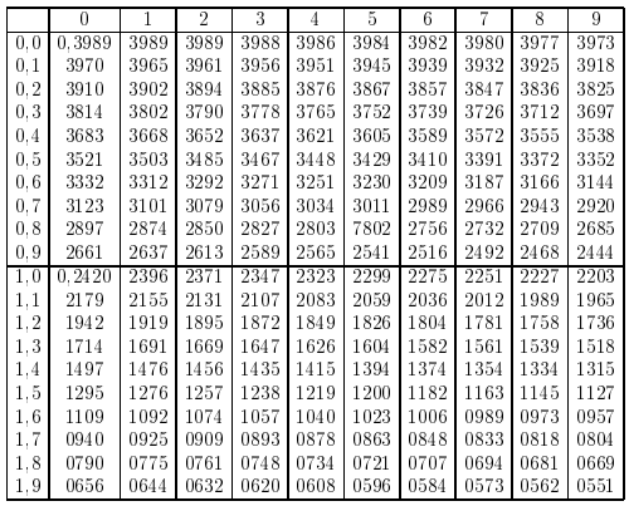
\includegraphics[width=0.85\textwidth]{images/gauss-table-1.png}
\end{center}
\begin{center}
  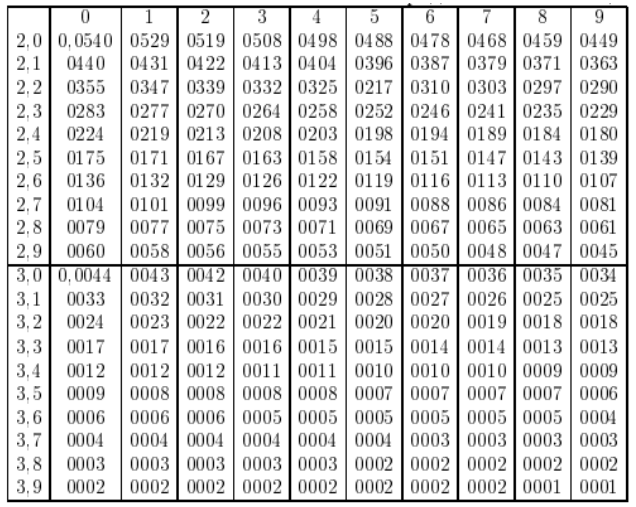
\includegraphics[width=0.85\textwidth]{images/gauss-table-2.png}
\end{center}

\newpage
\section{Таблица значений функции Лапласа}

Таблица значений функции Лапласа: $\Phi(x) = \frac{1}{\sqrt{2\pi}}\cdot \int\limits_{0}^{x} e^{-z^2/2}dz$

\begin{center}
  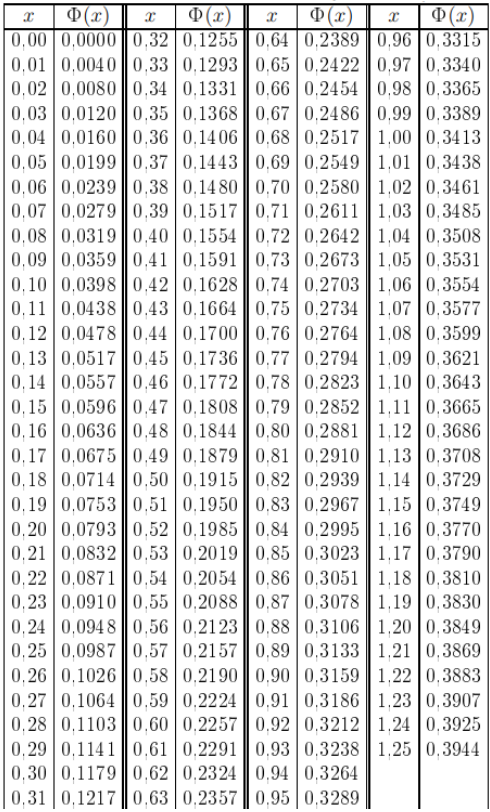
\includegraphics[width=0.8\textwidth]{images/laplas-table-1.png}
\end{center}
\begin{center}
  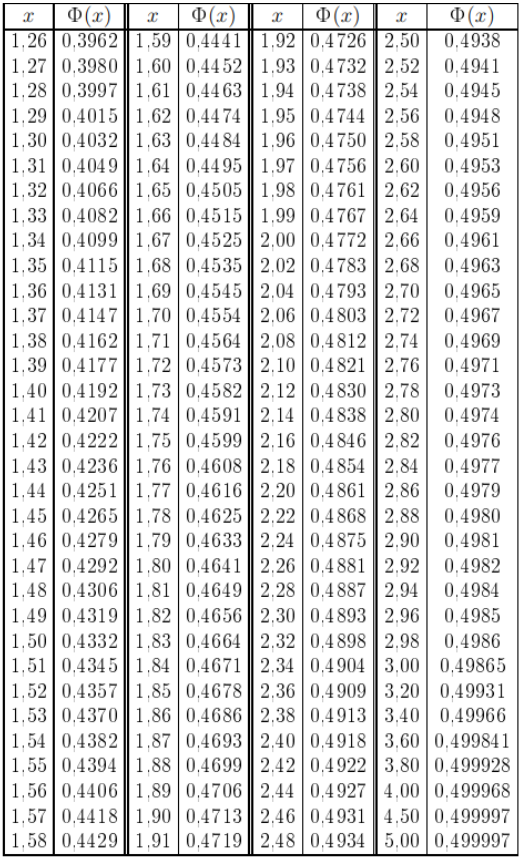
\includegraphics[width=0.85\textwidth]{images/laplas-table-2.png}
\end{center}


\end{document}
